\documentclass[thesis2.tex]{subfiles}

\begin{document}
\iffulldocument\else
	\chapter{KdV5}
\fi

\section{Numerical results}

In this section, we present numerical results for the existence and spectrum of solutions to \cref{KdV5c}. First, we construct the primary pulse solution for $c > 1/4$ using parameter continuation. We then use that  solution to construct multipulses and analyze the spectrum numerically. We perform time-stepping to see what the spectrum implies for the stability of multi-pulse solutions. Finally, we repeat these analyses for periodic multi-pulses for both small and extremely large periodic domains.

\subsection{Construction of single pulse}

We start with the construction of the primary pulse solution. For $c = 36/169 < 1/4$, an exact solution to \cref{KdV5eq4} is known \cite[(3)]{Pelinovsky2007}:
\begin{equation}\label{KdV5exactsol}
q(x) = \frac{105}{338}\sech^4\left(\frac{x}{2\sqrt{13}} \right)
\end{equation}

By \cite{Pelinovsky2007}, multi-pulses only exist when $c > 1/4$. To obtain a primary pulse solution for $c > 1/4$, we use AUTO for parameter continuation in $c$ starting with the solution \cref{KdV5exactsol} and $c = 36/169$. For a numerical scheme, we need to truncate the domain $\R$ to a bounded interval $[-L, L]$. In order to use AUTO, we scale equation \cref{KdV5eq4} from $[-L, L]$ to $[0, 1]$ by taking $x \mapsto \frac{1}{2L}(x + L)$. For the interval endpoints, we can use either periodic or separated (Dirichlet and Neumann at the endpoints) boundary conditions. As long the scaling is such that the tails of the primary pulse have adequate space to decay exponentially, it does not matter which boundary conditions we choose. For convenience, we will use periodic boundary conditions. Since \cref{KdV5eq4} is Hamiltonian, we will use the formulation \cref{KdV5ham2}; following the AUTO demo \texttt{kdv}, we include a small parameter $\epsilon$ to break the Hamiltonian structure. In \cref{fig:KdV5singlepulse}, we plot the exact solution (left) together with the output of parameter continuation for $c = 10$ (right). We note the presence of oscillatory tails for $c = 10$ (these are hard to see since the tails also decay exponentially, but the first downward bump is visible).
\begin{figure}
\begin{center}
\begin{tabular}{cc}
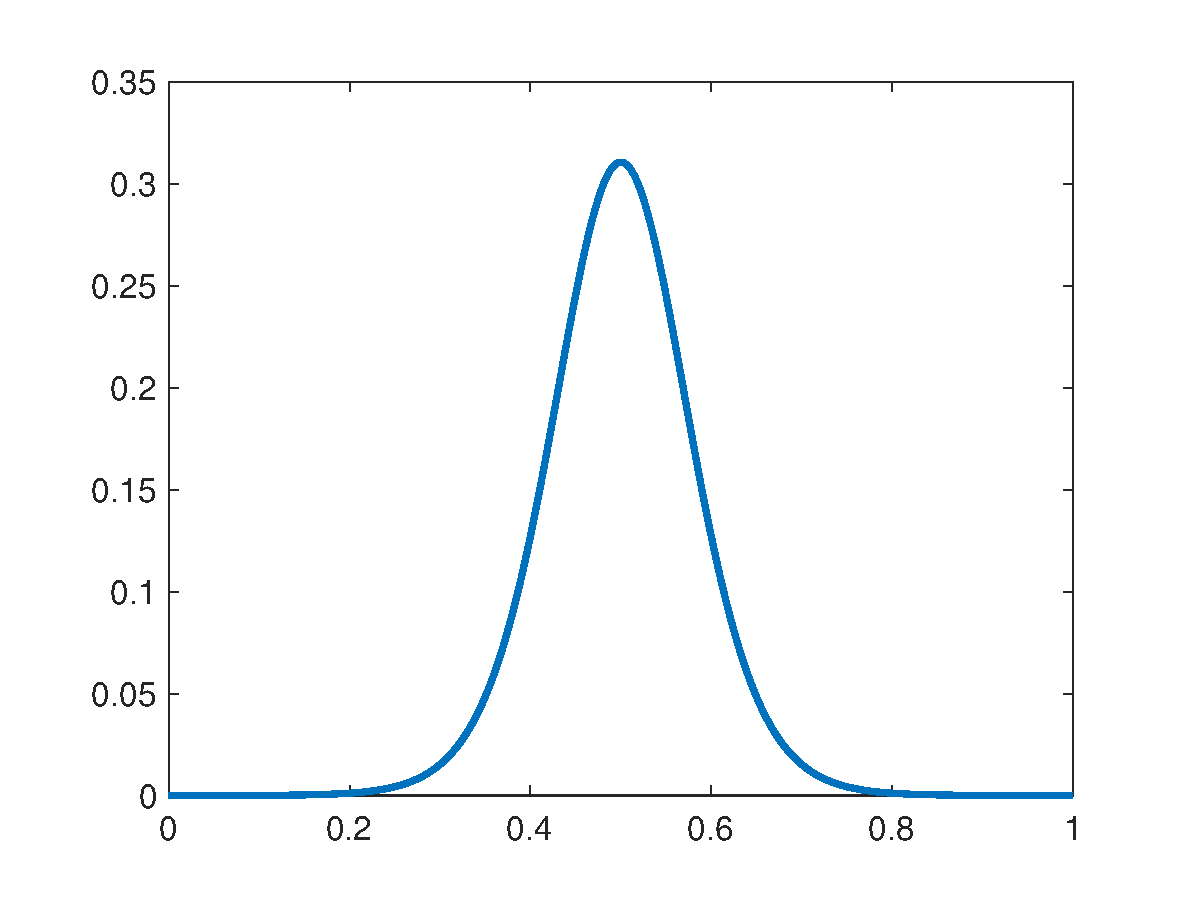
\includegraphics[width=8cm]{images/kdv5numerics/singleexact.eps} &
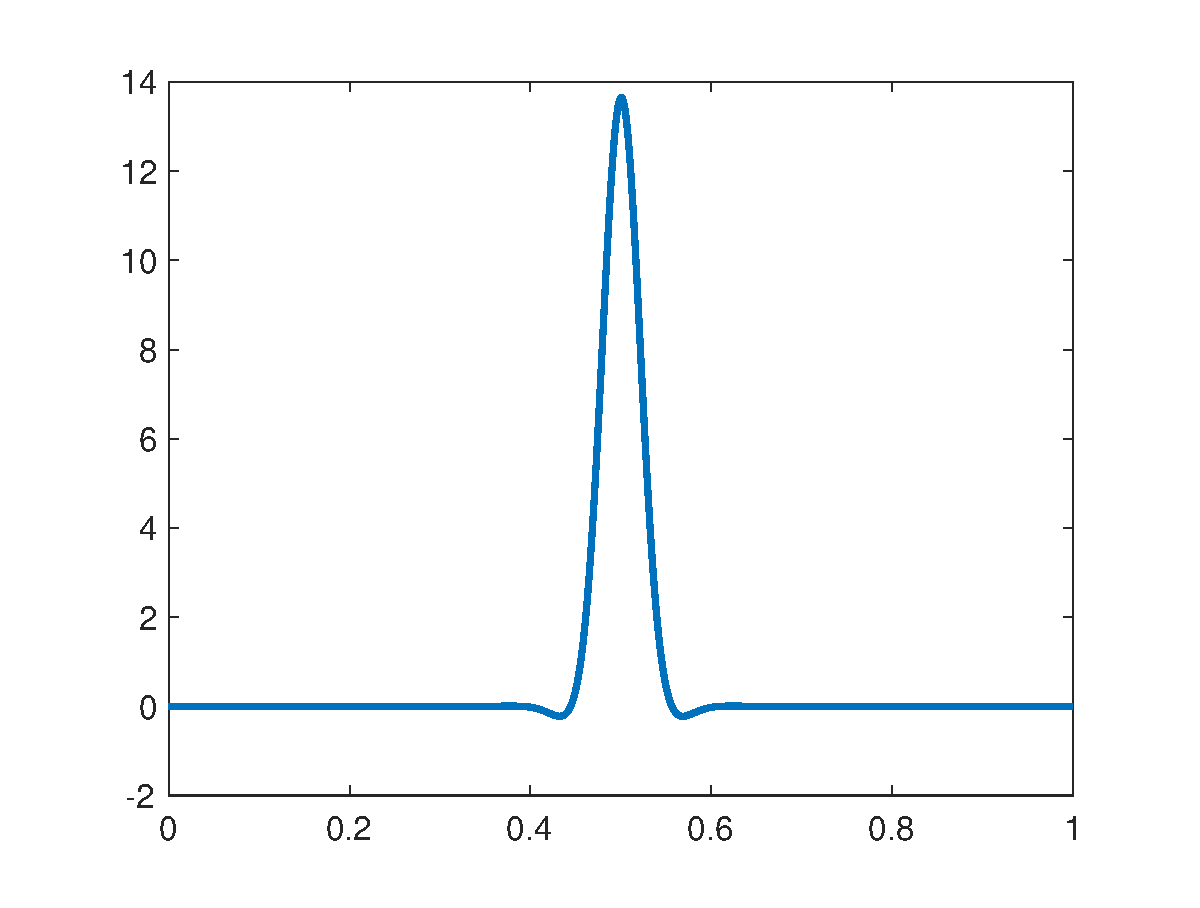
\includegraphics[width=8cm]{images/kdv5numerics/single10}
\end{tabular}
\caption[Primary pulse solutions for KdV5]{Single pulse solutions for KdV5. Exact solution for $c = 36/169$ (left) and solution from parameter continuation using AUTO for $c = 10.0$ (right). Solutions have been scaled to $[0, 1]$ using $L = 25$ in both cases.}
\label{fig:KdV5singlepulse}
\end{center}
\end{figure}

There is also a linear relationship between the height of the single pulse peak and the wavespeed $c$, as we can see in \cref{fig:KdV5peakht}.

\begin{figure}
\begin{center}
\includegraphics[width=8cm]{images/kdv5numerics/peakheightvsc}
\caption[Solitary wave amplitude vs. wavespeed for KdV5]{Plot of height of single pulse peak vs. wavespeed $c$. Dots are data points from numerical analysis, line is least squares linear regression line.}
\label{fig:KdV5peakht}
\end{center}
\end{figure}

\subsection{Construction of multi-pulses}\label{sec:kdv5nummulti}

To construct a multi-pulse, we glue together multiple copies of the single pulse we constructed in the previous section. For the peak distances, we use those predicted by \cite{SandstedeStrut}. For the spatial discretizaton of \eqref{KdV5eq4} we use either Fourier spectral methods with periodic boundary conditions or Chebyshev polynomial spectral methods with Dirichlet and Neumann boundary conditions at the endpoints. As long as the domain has sufficient room for the oscillatory tails to decay exponentially, it does not matter what method we use. In what follows, we use Fourier spectral methods. After the single pulses are spliced together, the multi-pulse is found using Matlab's \texttt{fsolve} function (Levenberg–Marquardt algorithm). The first six double pulse solutions are shown in \cref{fig:KdV5doublepulse}.

\begin{figure}
\begin{center}
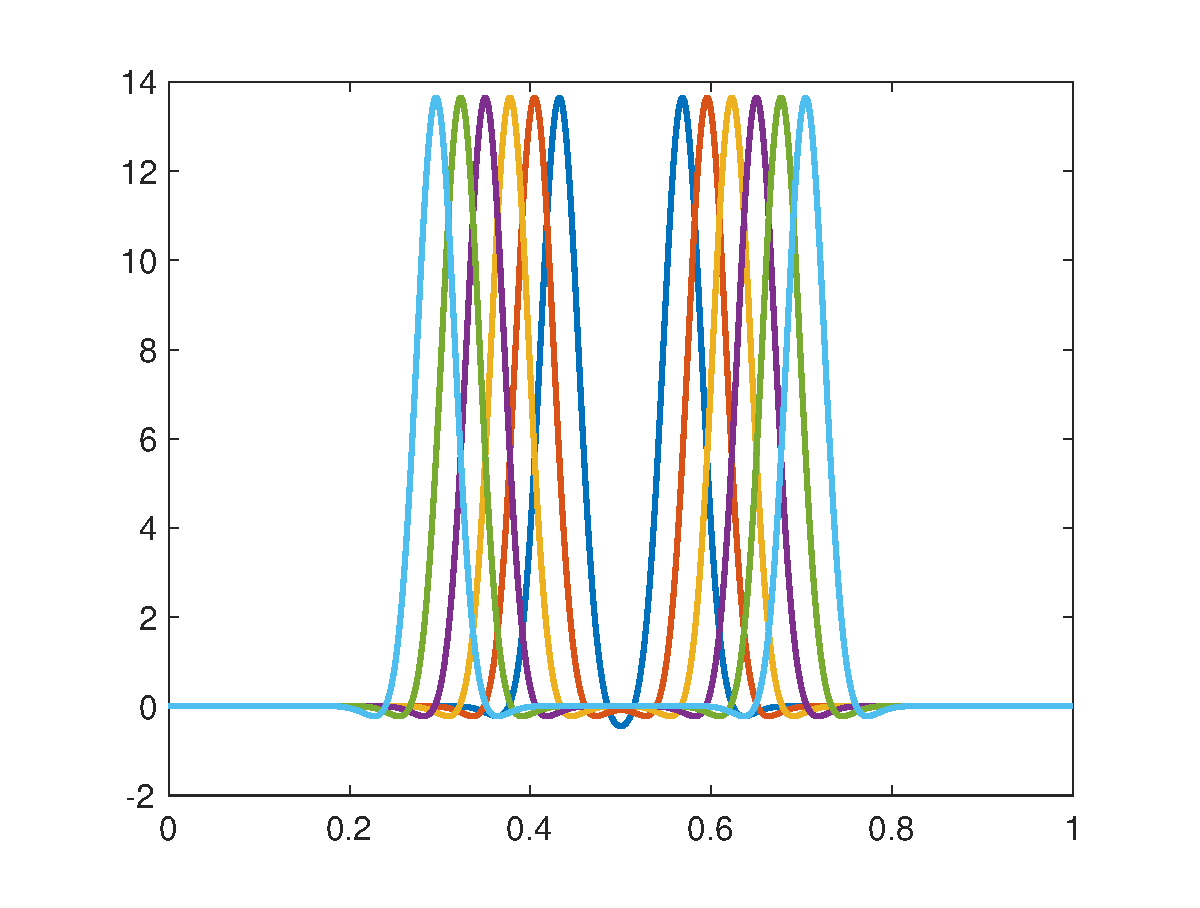
\includegraphics[width=8cm]{images/kdv5numerics/double10.eps}
\caption[Double pulse solutions for KdV5]{First six double pulse solutions for KdV5. Fourier spectral methods with $N = 1024$ grid points, $c = 10$, $L = 25$.}
\label{fig:KdV5doublepulse}
\end{center}
\end{figure}

This procedure can be used to construct arbitrary multi-pulses. Several of these are shown in \cref{fig:KdV5multipulse}.

\begin{figure}
\begin{center}
\begin{tabular}{cc}
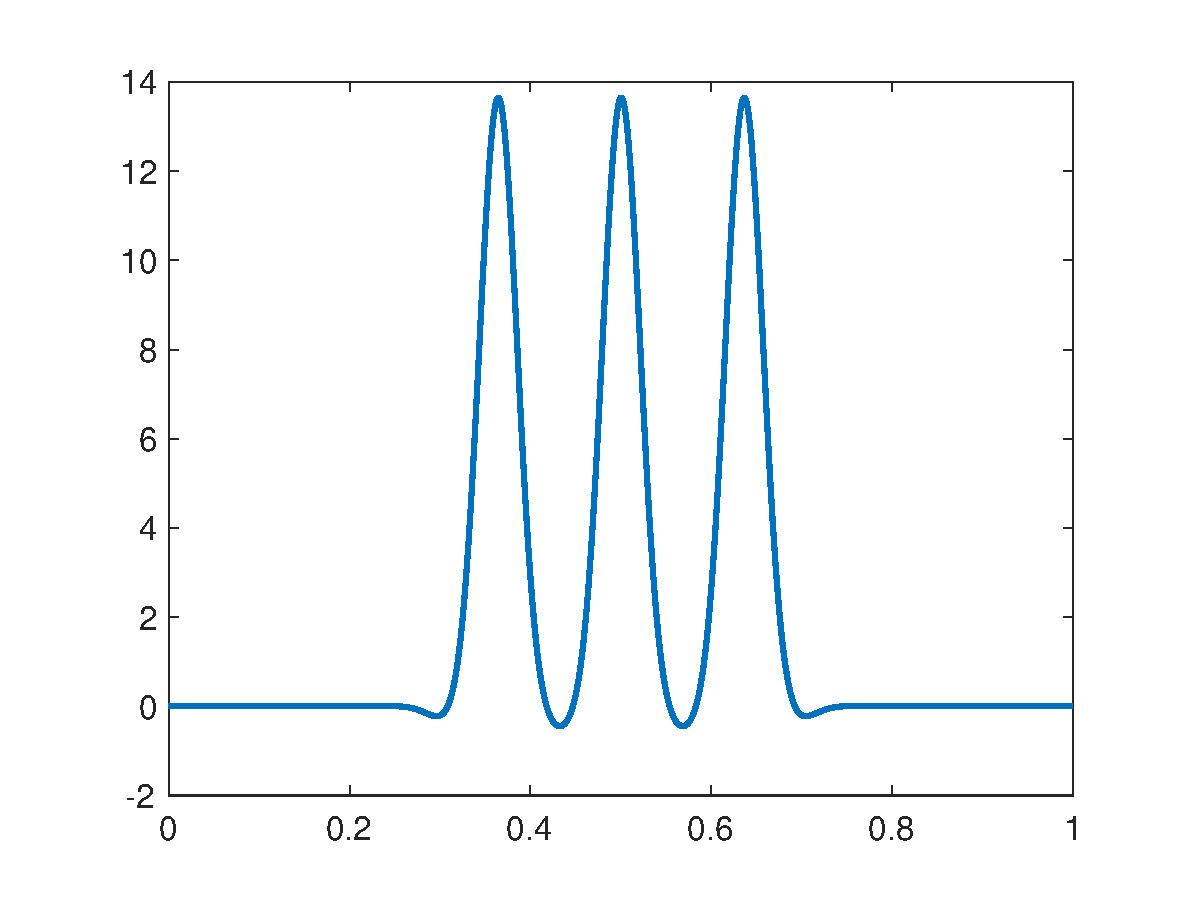
\includegraphics[width=6cm]{images/kdv5numerics/triple00} &
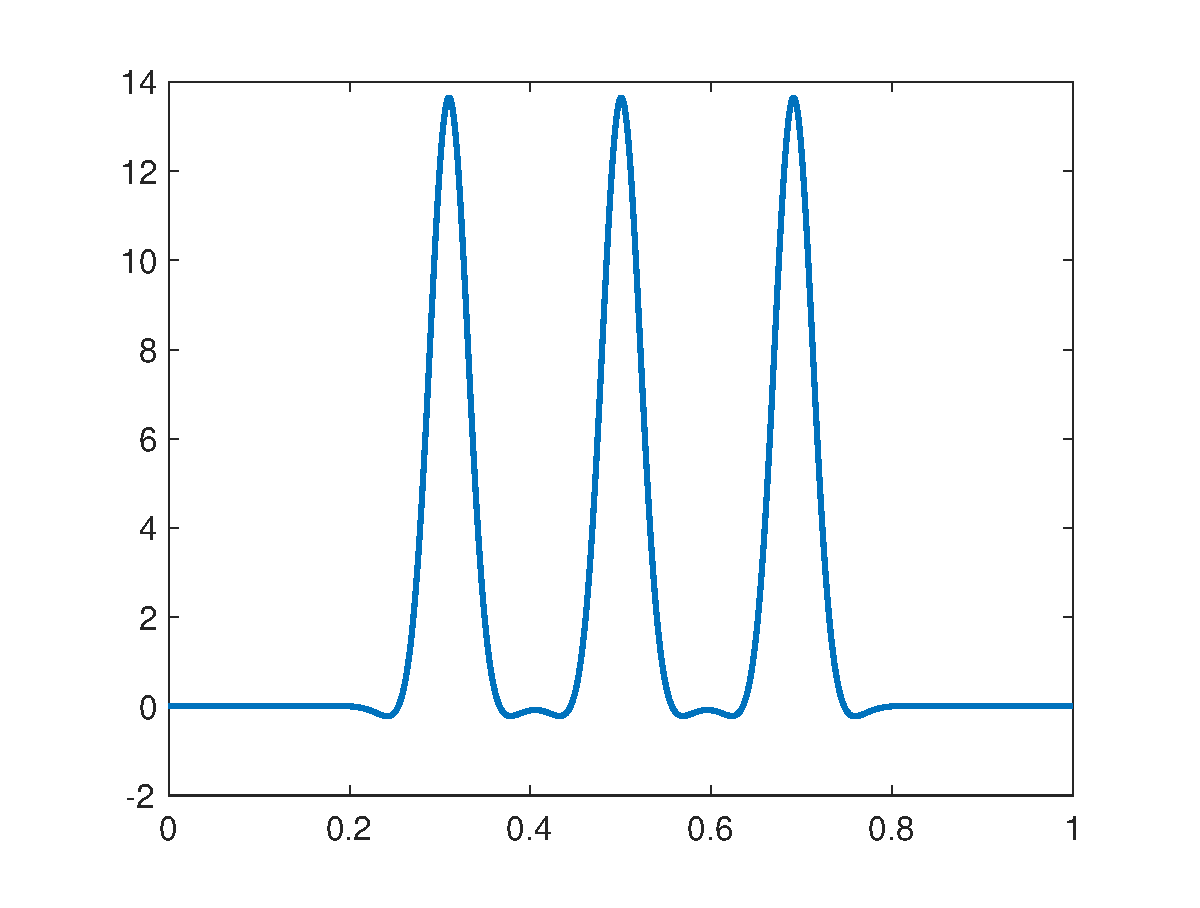
\includegraphics[width=6cm]{images/kdv5numerics/triple11} \\
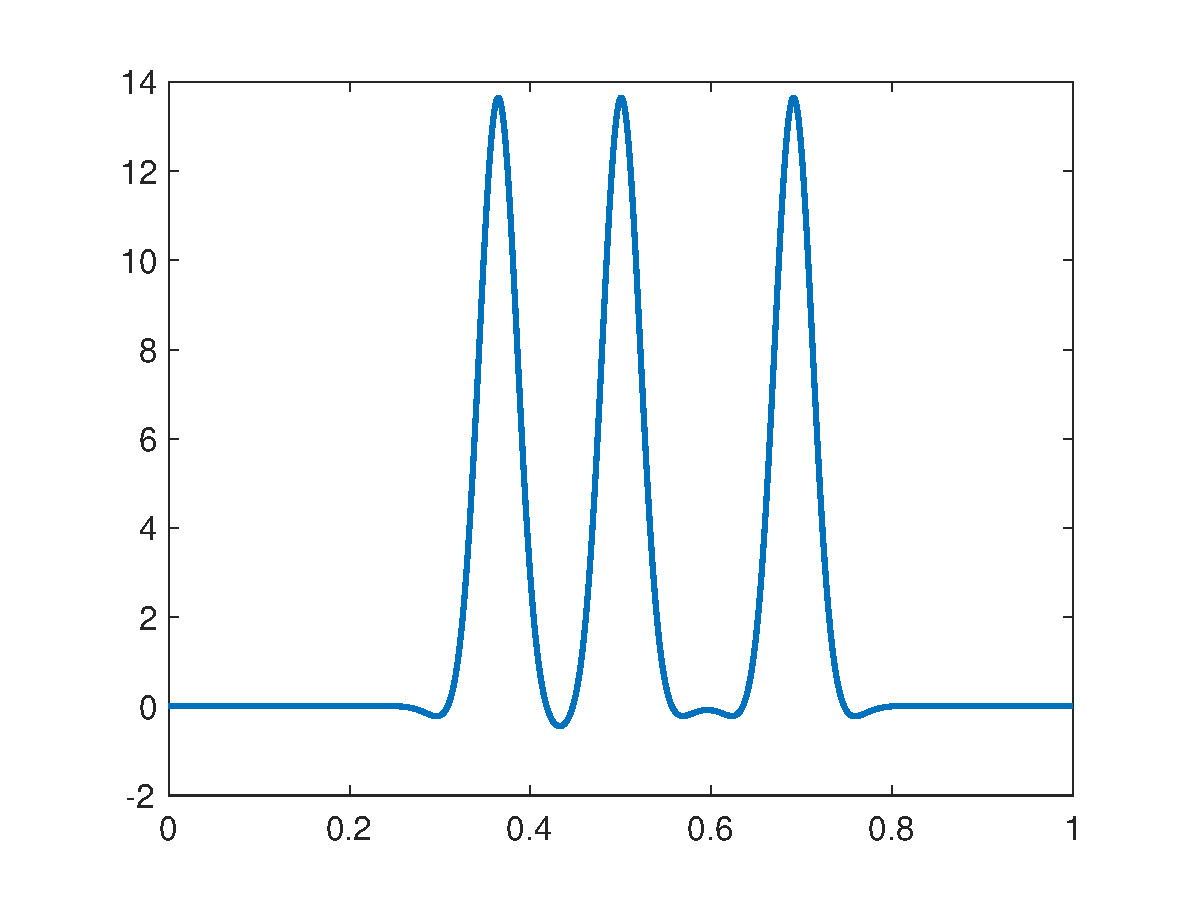
\includegraphics[width=6cm]{images/kdv5numerics/triple01} &
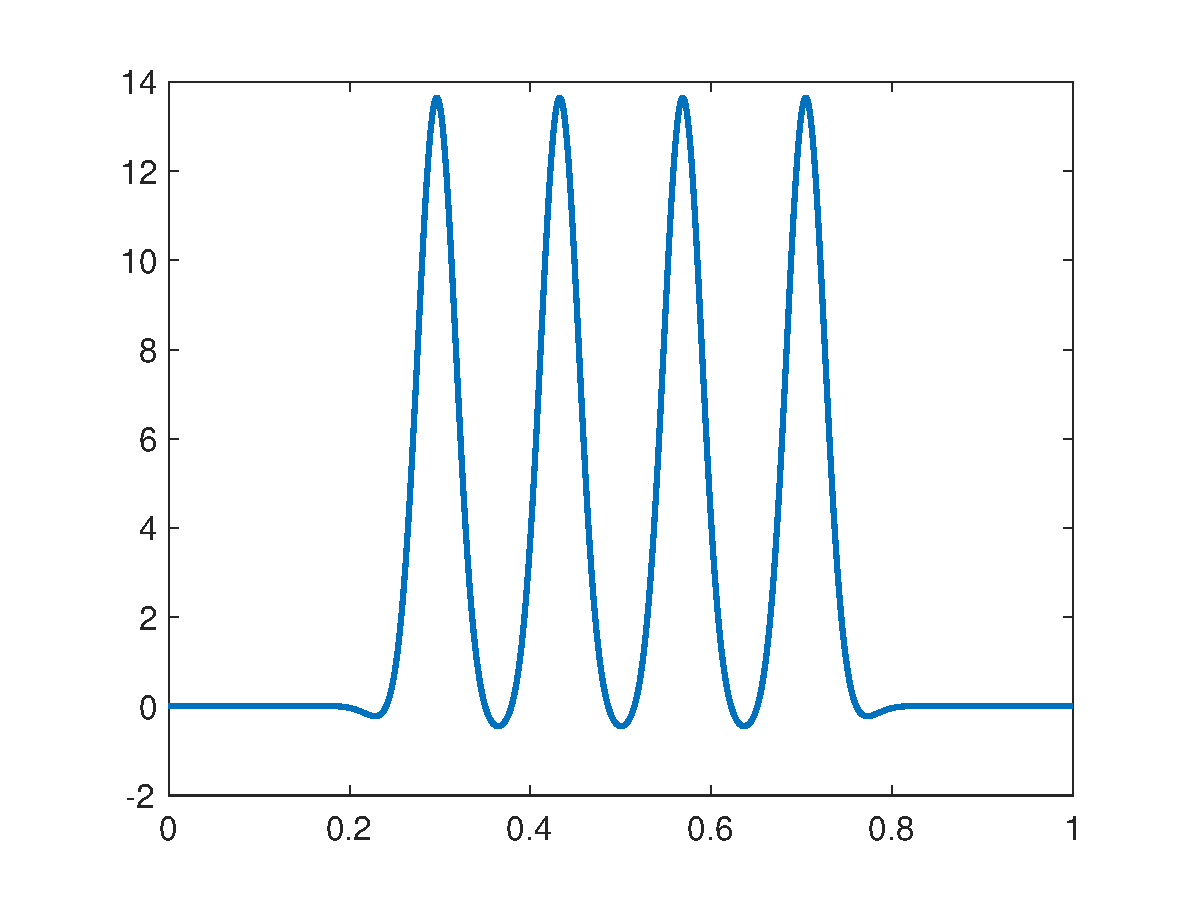
\includegraphics[width=6cm]{images/kdv5numerics/quad000} \\
\end{tabular}
\caption[Multi-pulse solutions for KdV5]{Multi-pulse solutions for KdV5. Symmetric triple pulses (top), asymmetric triple pulse (bottom left), and symmetric quadruple pulse (bottom right). Fourier spectral methods with $N = 1024$ grid points, $c = 10$, $L = 25$.}
\label{fig:KdV5multipulse}
\end{center}
\end{figure}

\subsection{Spectrum of multi-pulses}

Now that we have constructed multi-pulses, we can look at their spectral stability. For an $n$-pulse $q_n$, we compute the spectra of $\calE''(q_n)$ and $\partial_x \calE''(q_n)$ numerically by writing the linear operator in matrix form using differentiation matrices and computing the eigenvalues of the resulting matrix using Matlab's \texttt{eig} function. Since $\calE''(q_n)$ is self-adjoint, its eigenvalues will be real. For an $n$-pulse, we expect to have $n$ eigenvalues $\{ \mu_1, \dots, \mu_{n-1}, 0 \}$ close to 0. The last one is always 0 from the kernel eigenfunction $\partial_x q_n$. The remaining $n-1$ eigenvalues $\{\mu_1, \dots, \mu_{n-1}\}$ will be close to 0 but nonzero. The operator $\calE''(q_n)$ will also have $n$ negative eigenvalues which are located well away from 0; we will not be showing these in our plots. We expect that $\partial_x \calE''(q_n)$ will have $n-1$ pairs of interaction eigenvalues, which are either real or purely imaginary. Each positive eigenvalue $\mu_j$ of $\calE''(q_n)$ will correspond to a pair of real eigenvalues of $\partial_x \calE''(q_n)$, and each negative eigenvalue $\mu_j$ of $\calE''(q_n)$ will correspond to a pair of purely imaginary eigenvalues of $\partial_x \calE''(q_n)$. Furthermore, we expect that the interaction eigenvalues are related to the eigenvalues $\mu_j$ of $\calE''(q_n)$ by $\lambda_j = \pm C \sqrt{\mu_j}$ for some constant $C$. See \cref{remark:eigrelation} for more details.

We start by looking at double pulses $q_2$. \cref{fig:KdV5doublespec} shows the two spectra for the first four double pulses.
\begin{figure}
\begin{center}
\begin{tabular}{cc}
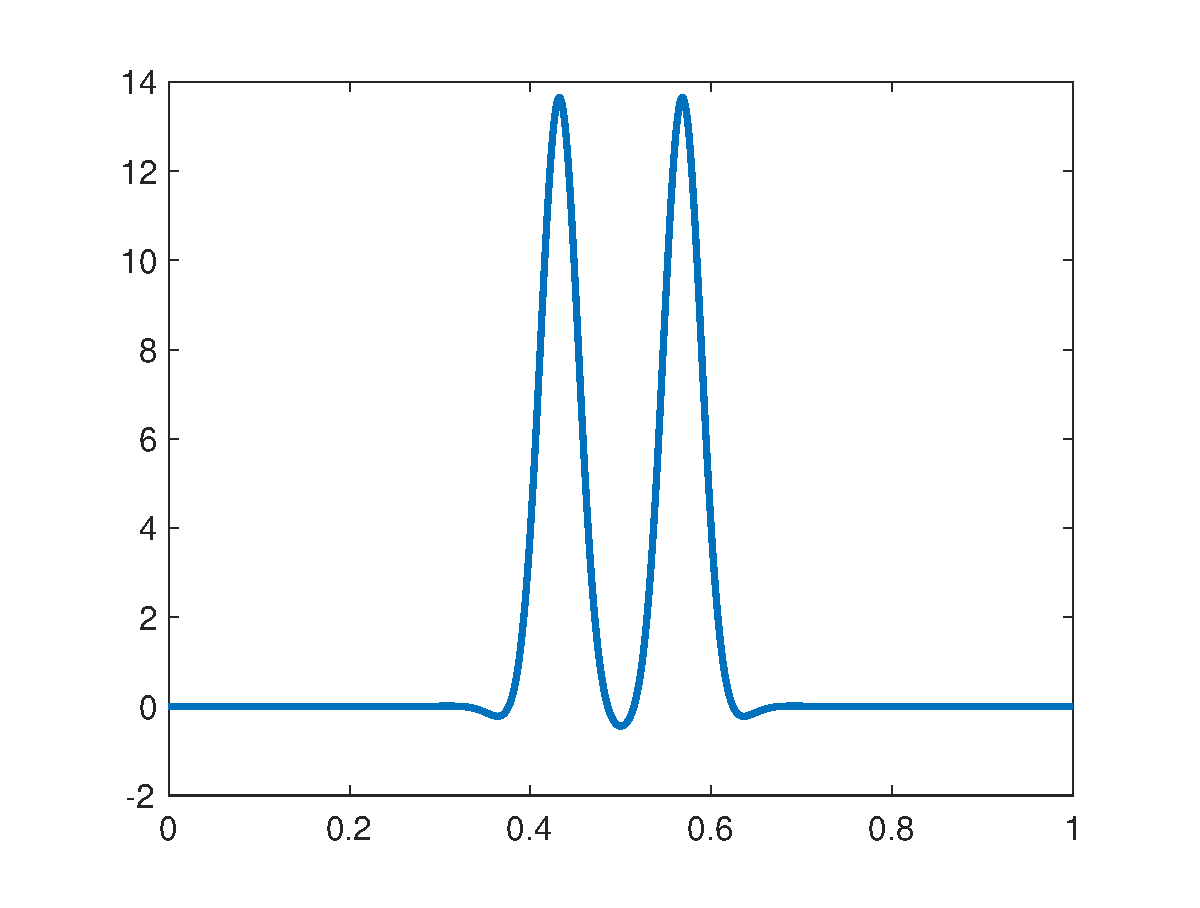
\includegraphics[width=5cm]{images/kdv5numerics/double1} &
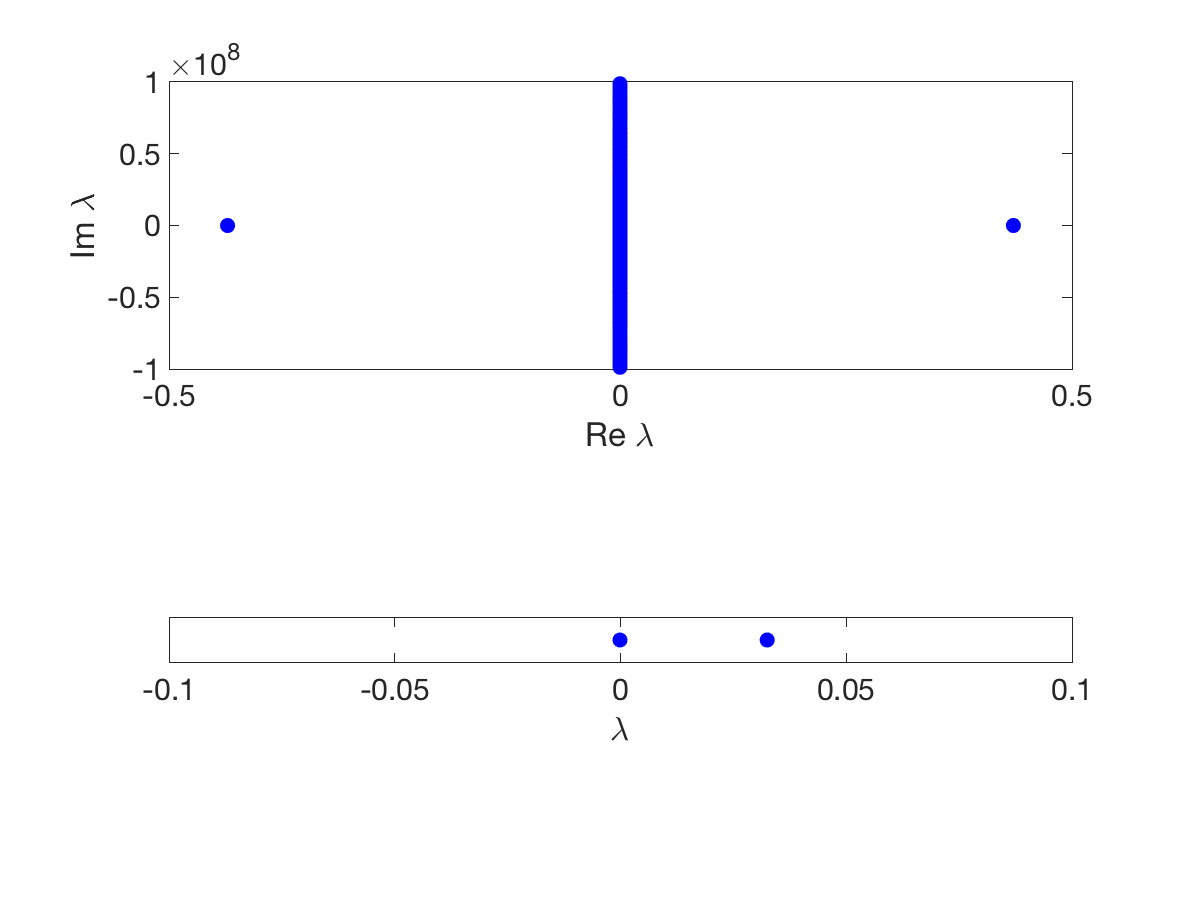
\includegraphics[width=5cm]{images/kdv5numerics/double1spec} \\
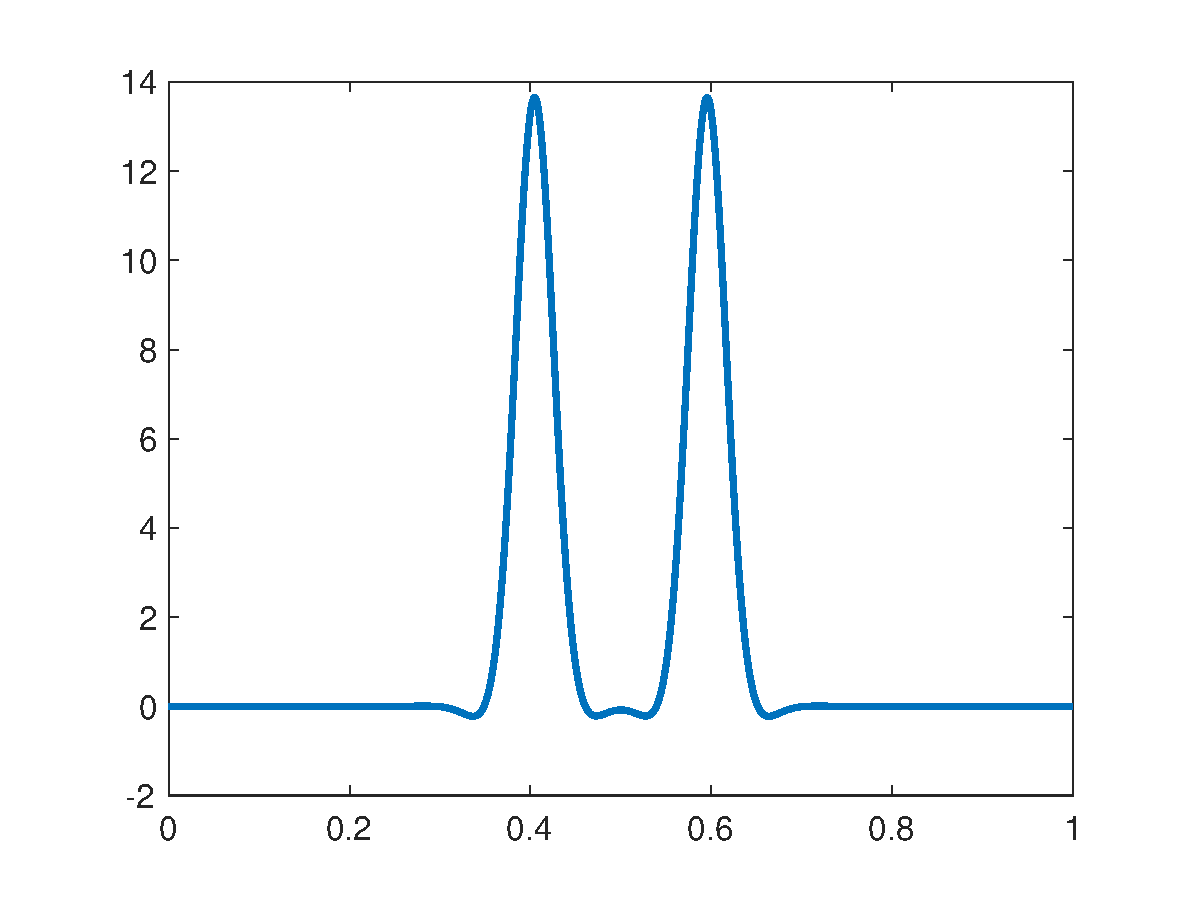
\includegraphics[width=5cm]{images/kdv5numerics/double2} &
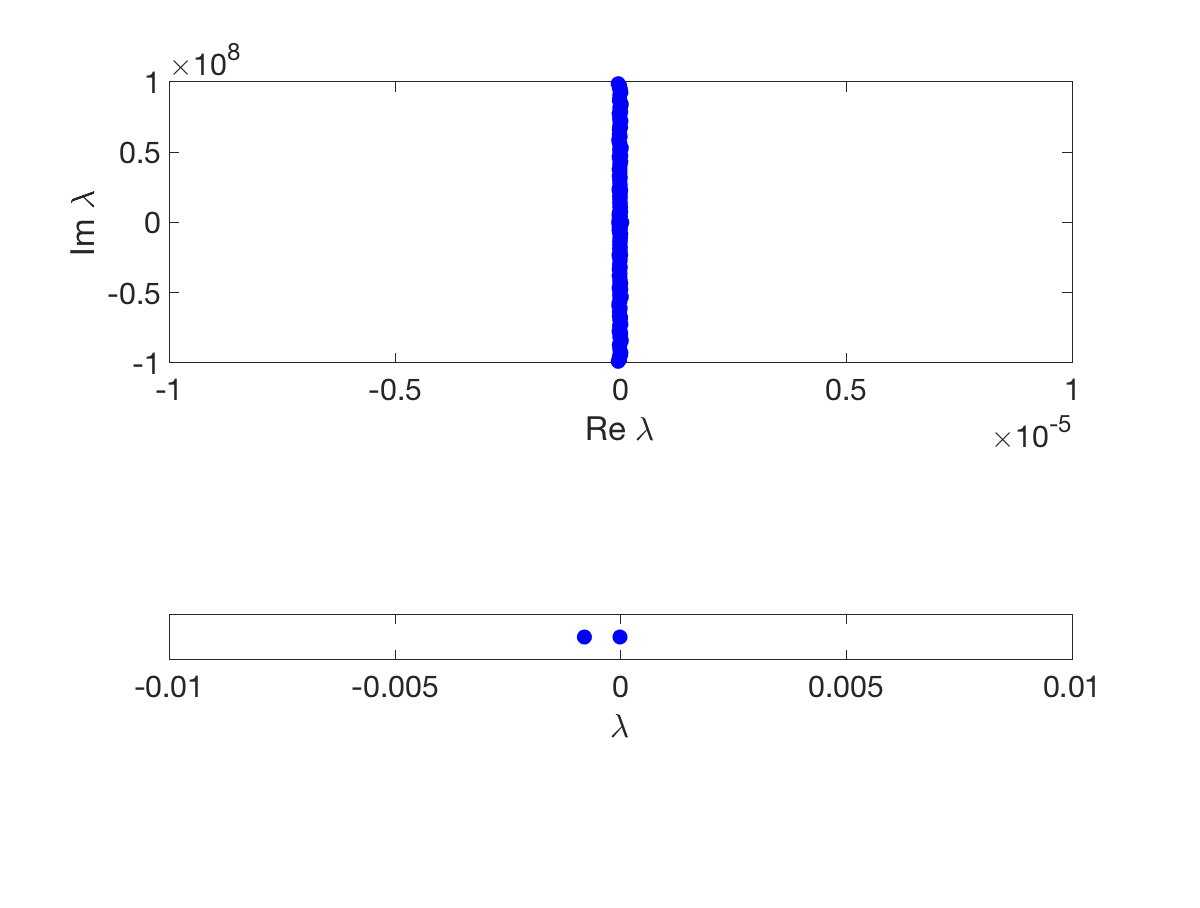
\includegraphics[width=5cm]{images/kdv5numerics/double2spec} \\
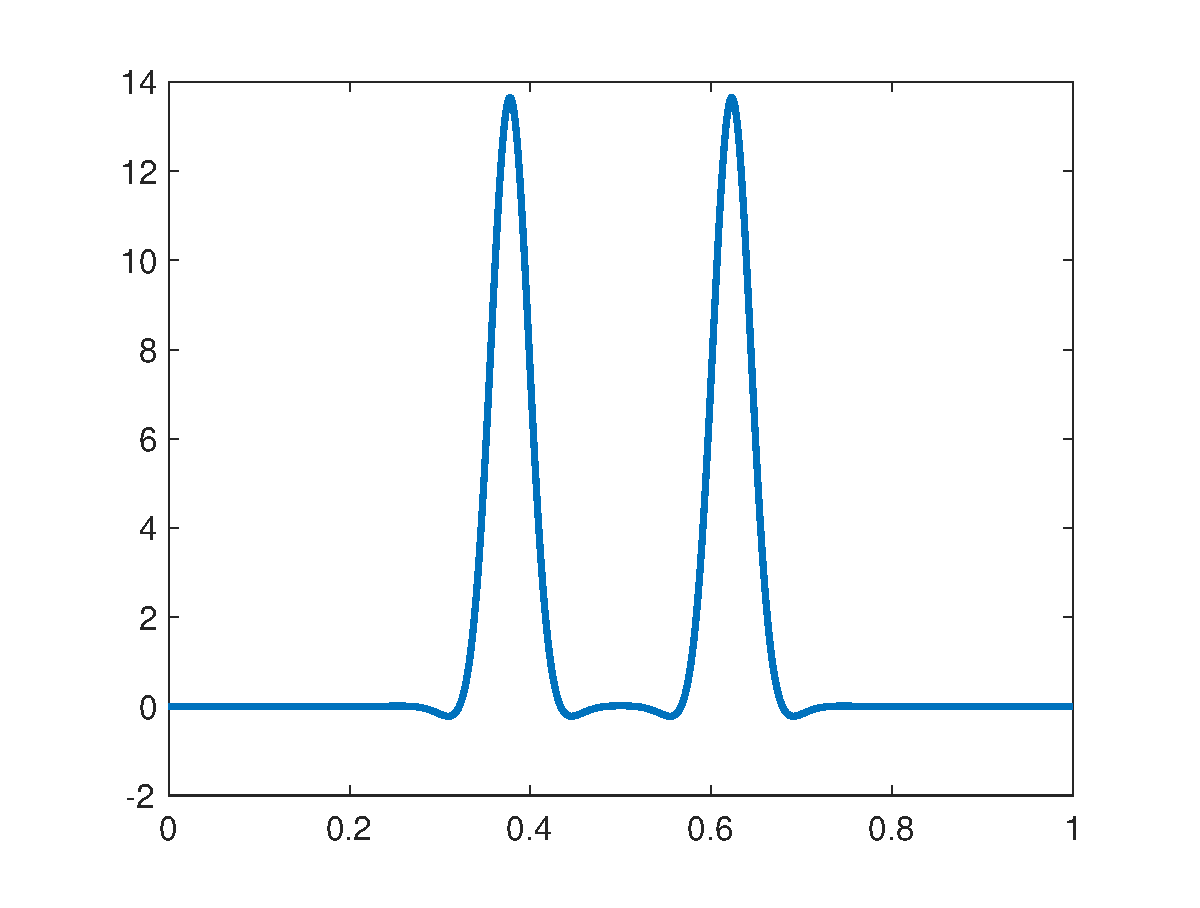
\includegraphics[width=5cm]{images/kdv5numerics/double3} &
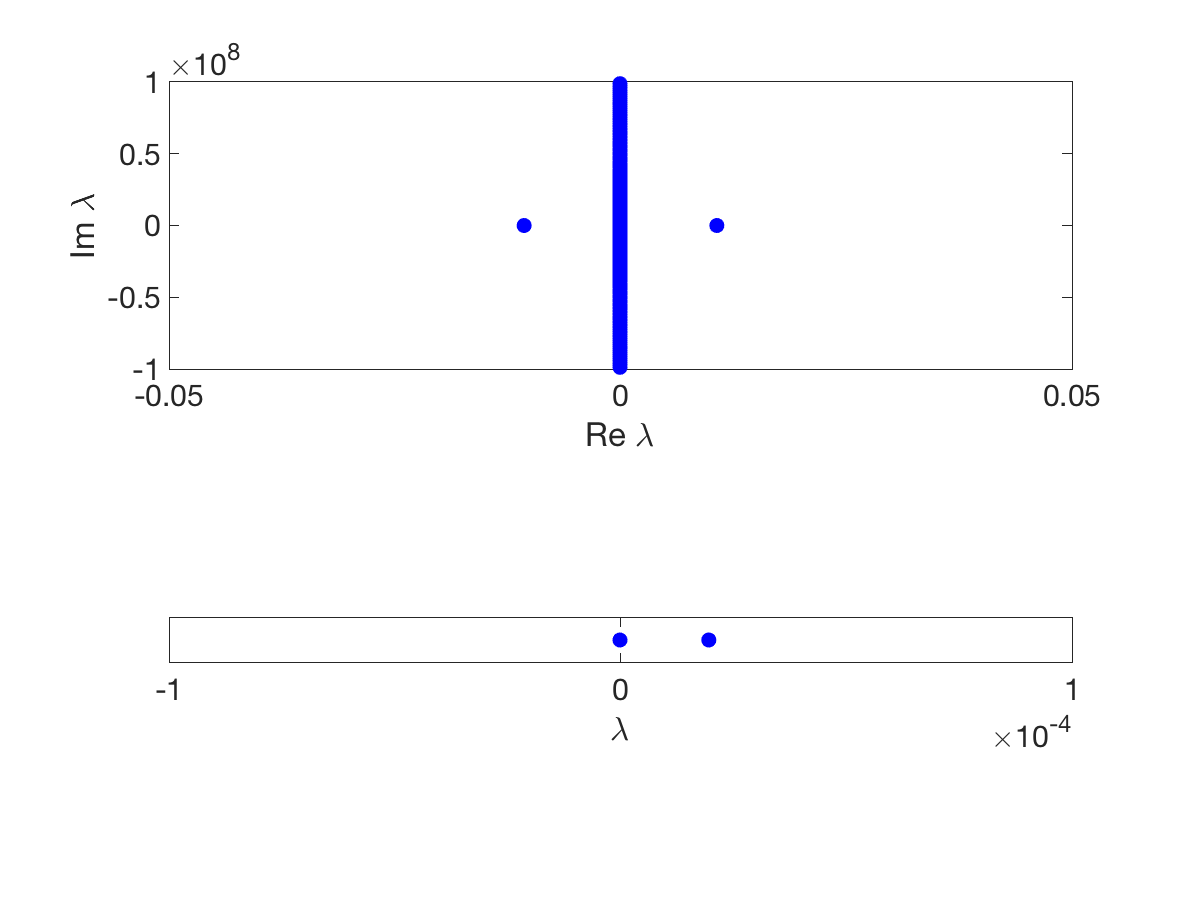
\includegraphics[width=5cm]{images/kdv5numerics/double3spec} \\
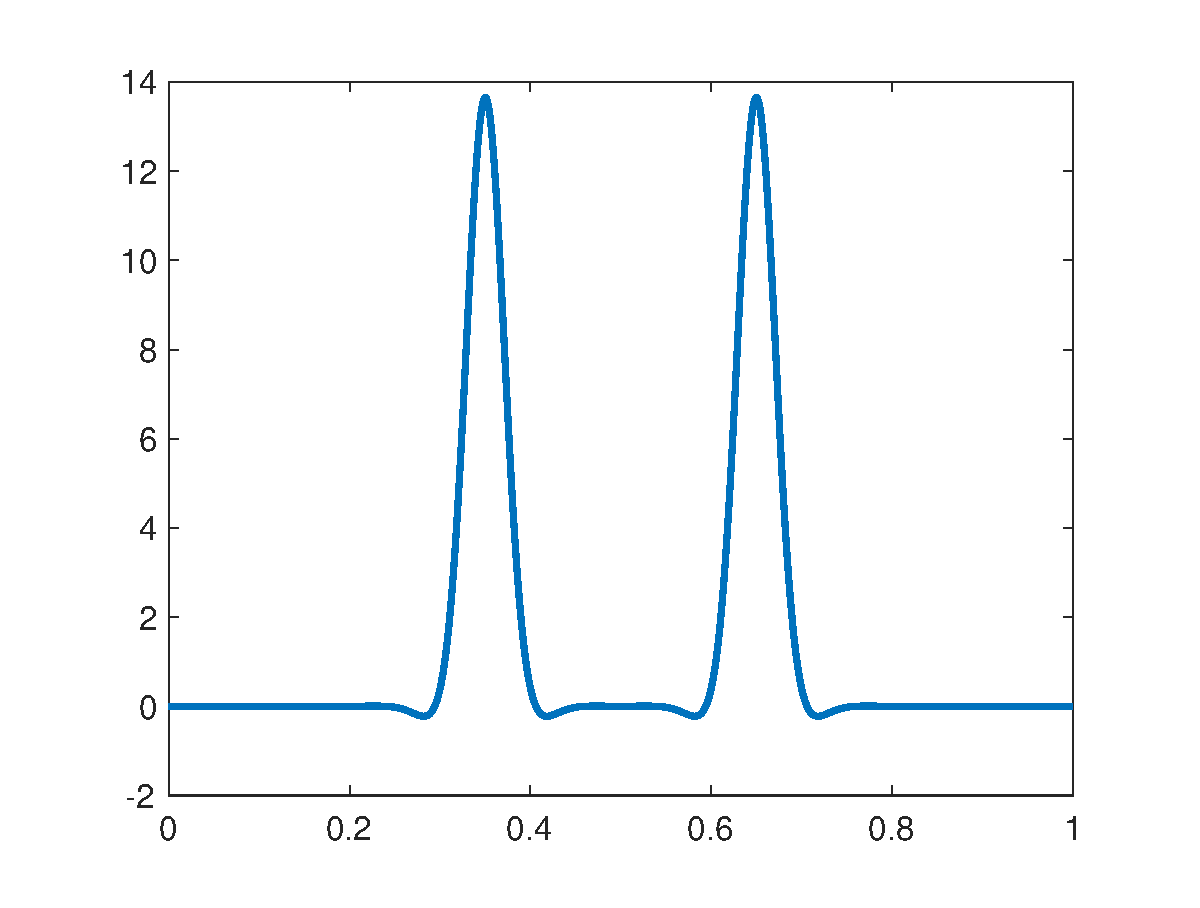
\includegraphics[width=5cm]{images/kdv5numerics/double4} &
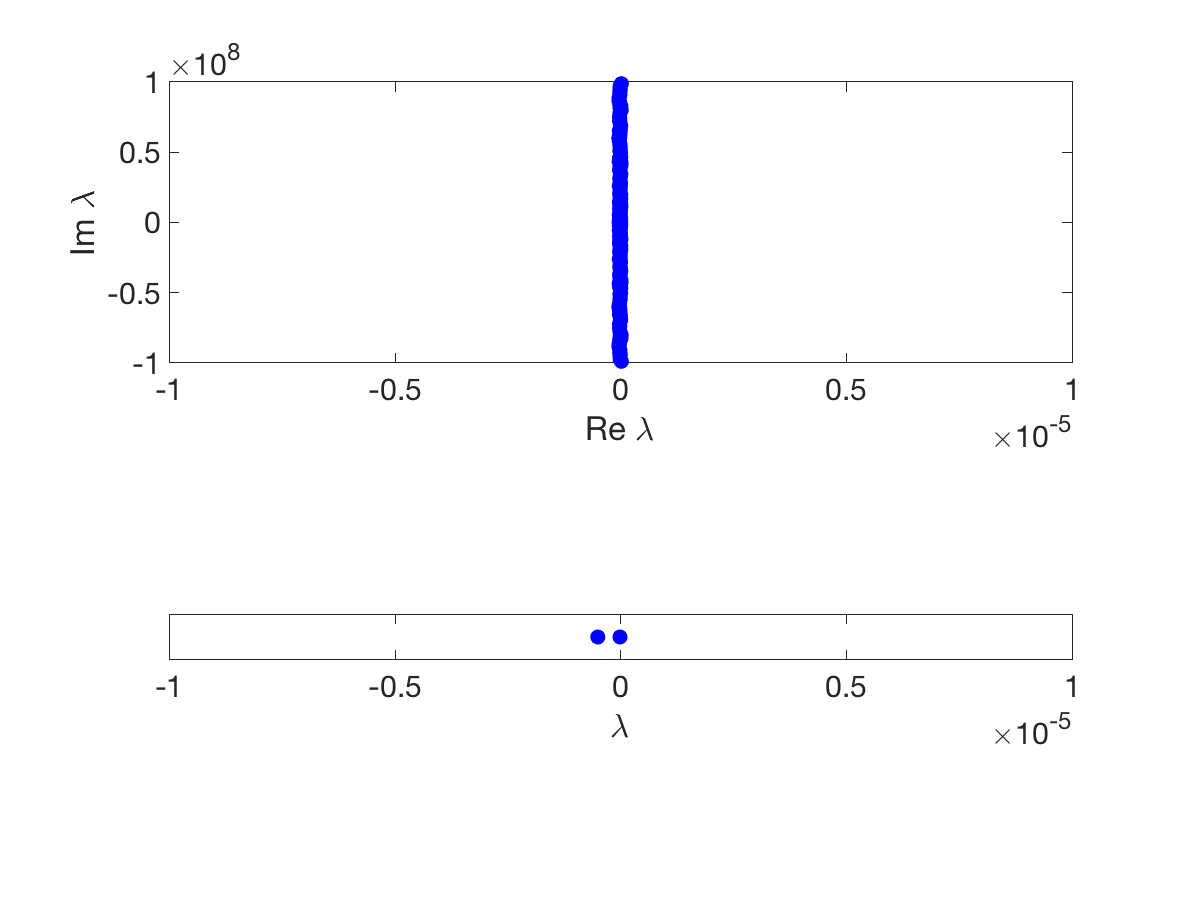
\includegraphics[width=5cm]{images/kdv5numerics/double4spec} \\
\end{tabular}
\caption[Spectrum of double pulses for KdV5]{Spectrum of $\calE''(q_2)$ and $\partial_x \calE
''(q_2)$ for the first four double pulses. For each row, the double pulse $q_2$ is shown on the left. The corresponding spectra are on the right; the spectrum of $\partial_x \calE''(q_2)$ near 0 is on the top and the spectrum of $\calE''(q_2)$ is on the bottom. Fourier spectral methods with $N = 1024$ grid points, $c = 10$, $L = 25$.}
\label{fig:KdV5doublespec}
\end{center}
\end{figure}
For the first and third double pulse, $\calE''(q_2)$ has a positive eigenvalue close to 0, and $\partial_x \calE''(q_2)$ has a pair of real interaction eigenvalues. For the second and fourth double pulse, $\calE''(q_2)$ has a small, negative eigenvalue. By \cite[Theorem 2.3]{Pelinovsky2007}, we expect that $\partial_x \calE''(q_2)$ has a pair of eigenvalues which are purely imaginary to leading order. We cannot see them in \cref{fig:KdV5doublespec}, however, since the essential spectrum is in the way. To locate these interaction eigenvalues, we shift to an exponentially weighted space, which will move the essential spectrum to the left but will leave the point spectrum unchanged. We can then search for these eigenvalues in the spectrum of the unweighted problem. The interaction eigenvalues for the first four double pulses are listed in \cref{table:KdV5inteigs}.

\begin{table}
\centering
\begin{tabular}{|c|c|} 
 \hline
 Double Pulse & Interaction Eigenvalues \\
 \hline
 1 & $\pm 0.4351$ \\
 2 & $-2.107\text{e-}09 \pm 0.0678 i$ \\
 3 & $\pm 0.0107$ \\
 4 & $1.339\text{e-}08 \pm 0.00169 i$ \\
 \hline
\end{tabular}
\caption[Interaction eigenvalues for double pulses for KdV5]{Interaction eigenvalues for first four double pulses computed with \texttt{eig}. Fourier spectral methods with $N = 1024$ grid points, $c = 10$, $L = 25$.}
\label{table:KdV5inteigs}
\end{table}

The odd numbered double pulses have real eigenvalues, as expected. The even numbered double pulse have a pair of eigenvalues which are purely imaginary to leading order, which confirms the result of \cite[Theorem 2.3]{Pelinovsky2007}. It is likely, however, that these eigenvalues are in fact purely imaginary. The evidence in favor of this is as follows. First, the real part is very small, although not quite machine error. The sign of the small real part is also arbitrary. In addition, because of Hamiltonian symmetry, if there were a small real part we would expect to see a quartet of eigenvalues, which does not occur. Finally, we can use Matlab's \texttt{fsolve} function to construct an ``improved'' eigenfunction for which the eigenvalue is purely imaginary and the residual $|E''(q_2)v - \lambda v|$ is smaller.

To determine how the magnitude of the interaction eigenvalue $\lambda$ decays as the distance $X$ between pulses increases, we plot $\log |\lambda|$ versus $X$ in \cref{fig:KdV5doubleeigdecay}. 
\begin{figure}
\begin{center}
\includegraphics[width=8cm]{images/kdv5numerics/doubleeigdecay.eps}
\caption[Scaling of interaction eigenvalues for KdV5]{Plot of $\log |\lambda|$ versus the inter-pulse distance for the first four double pulses together with least squares linear regression line.}
\label{fig:KdV5doubleeigdecay}
\end{center}
\end{figure}
The slope of the least squares linear regression line is within $0.005$ of $\alpha_0/2$, which suggests that the interaction eigenvalues for the double pulse have magnitude
\[
|\lambda| = C e^{-\alpha_0 X/2}
\] 
We can also look at the eigenvalues for other multi-pulses. The spectra of $\calE''(q_2)$ and $\partial_x \calE''(q_2)$ for the multi-pulses in \cref{fig:KdV5multipulse} are shown in \cref{fig:KdV5multipulsespectra}. 
\begin{figure}
\begin{center}
\begin{tabular}{cc}
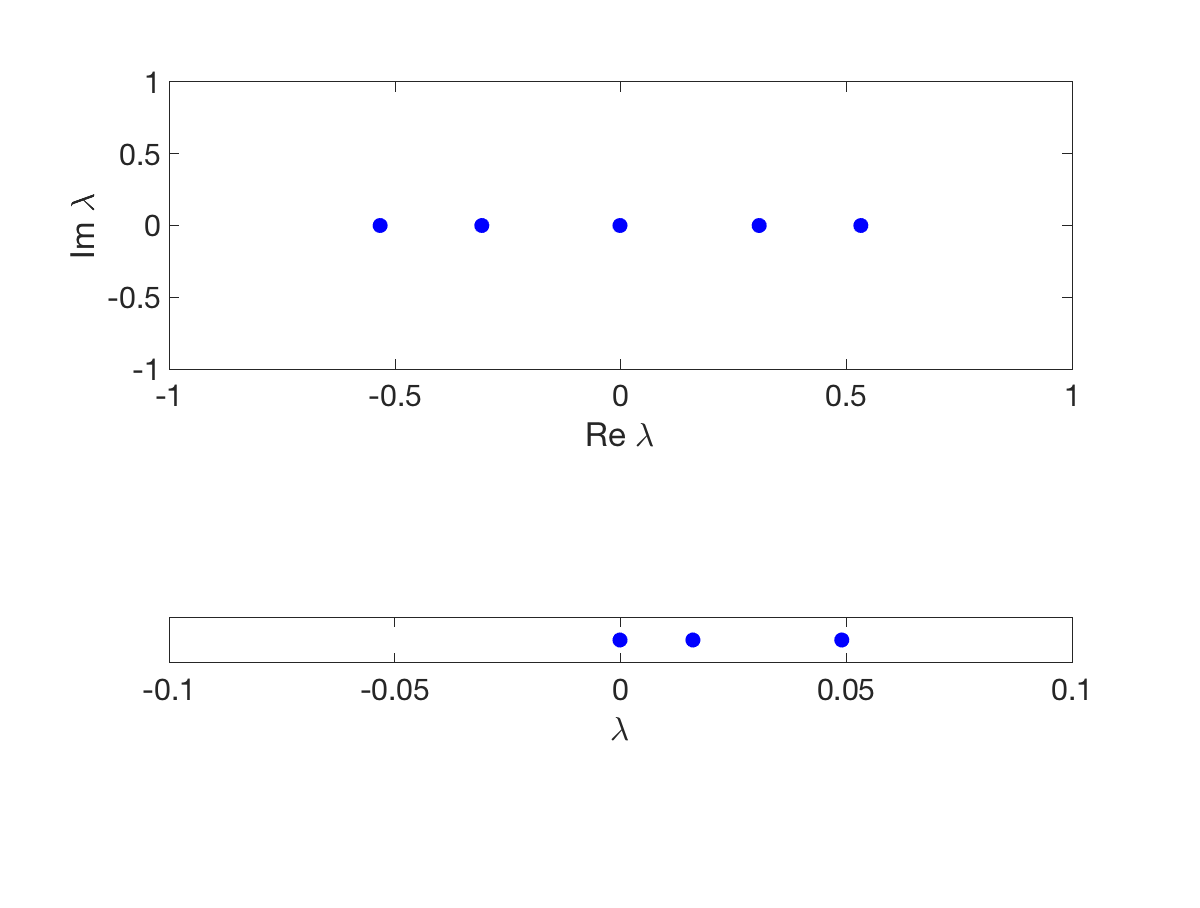
\includegraphics[width=7cm]{images/kdv5numerics/triple00spec} &
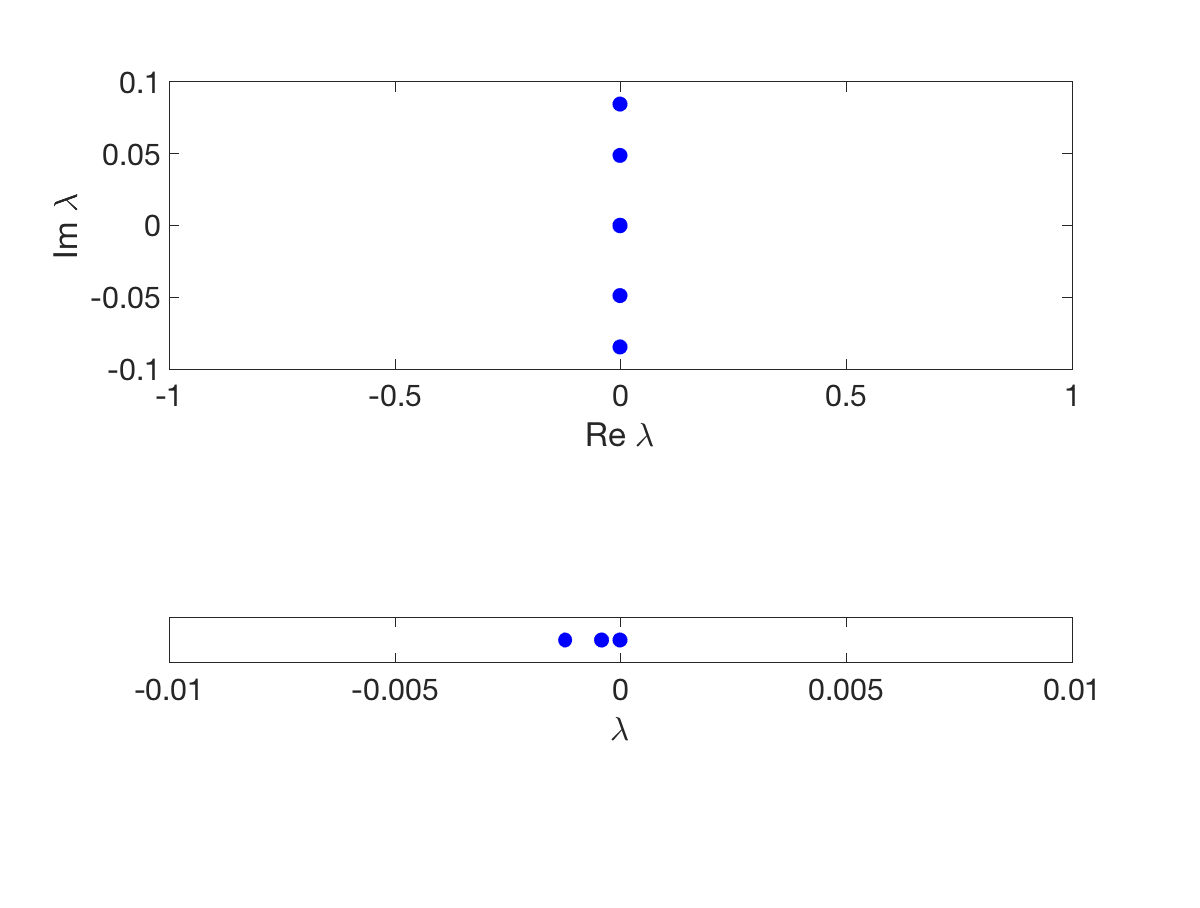
\includegraphics[width=7cm]{images/kdv5numerics/triple11spec} \\
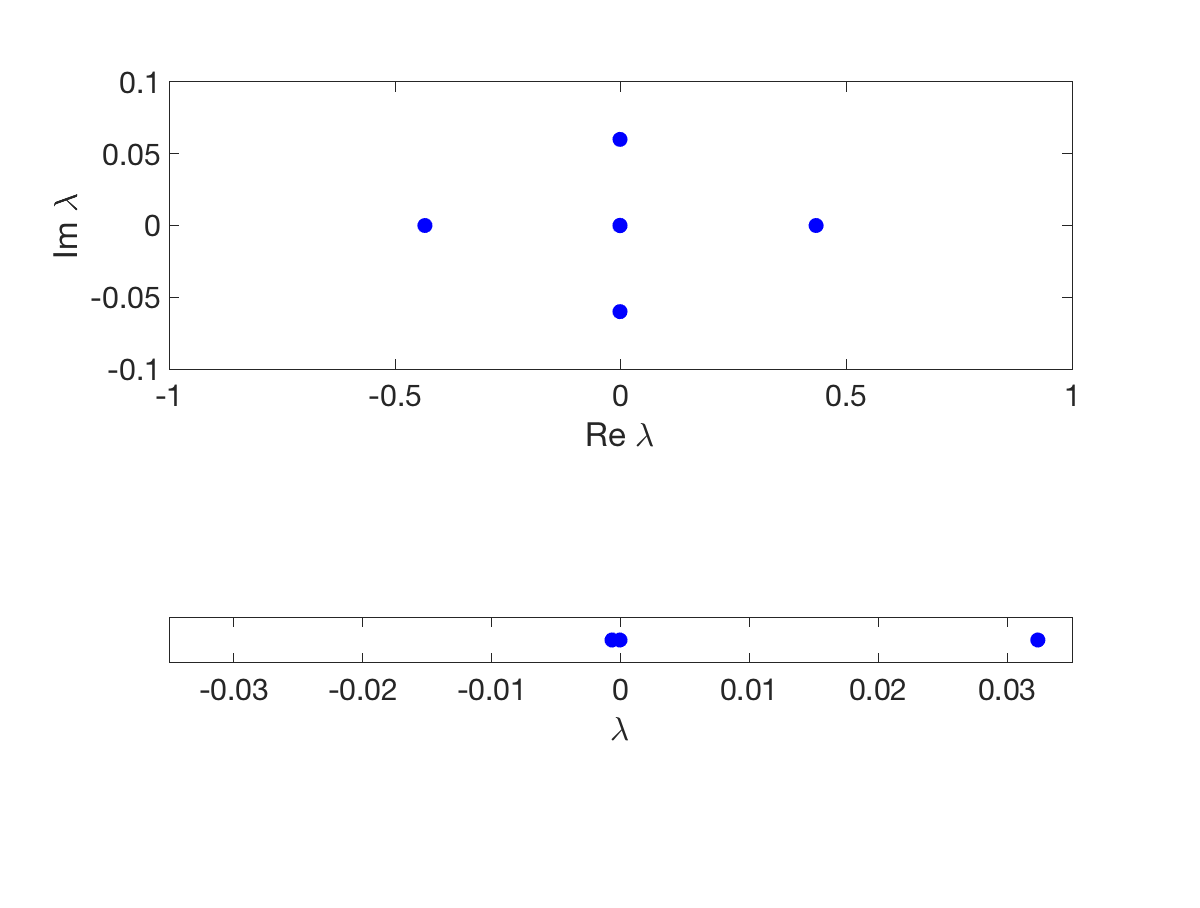
\includegraphics[width=7cm]{images/kdv5numerics/triple01spec} &
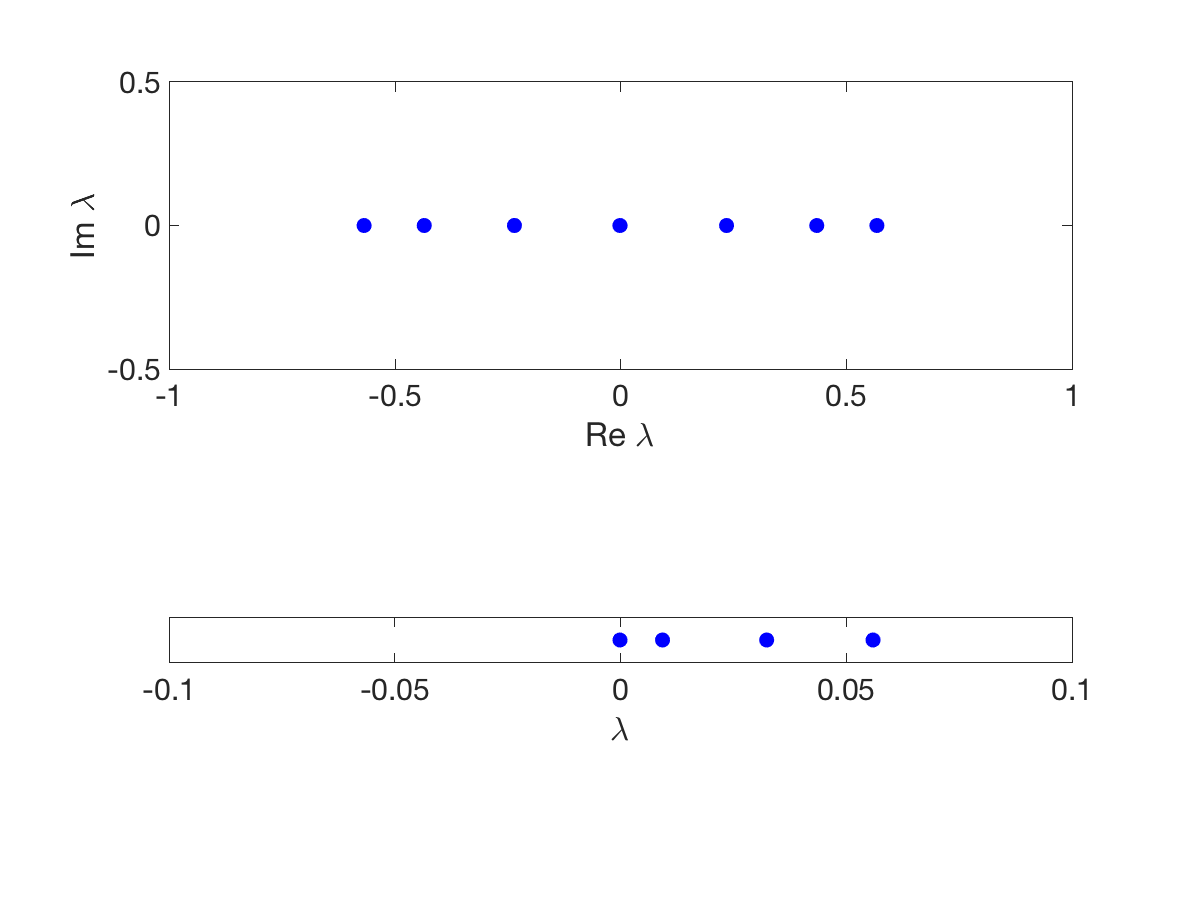
\includegraphics[width=7cm]{images/kdv5numerics/quad000spec} \\
\end{tabular}
\caption[Spectrum of multi-pulses for KdV5]{Spectra of $\calE''(q_2)$ and $\partial_x \calE''(q_2)$ for the multi-pulse solutions in \cref{fig:KdV5multipulse}. In each quadrant, spectrum of $\partial_x \calE''(q_2)$ is on the top and spectrum of $\calE''(q_2)$ is on the bottom. Symmetric triple pulses (top), asymmetric triple pulse (bottom left), and symmetric quadruple pulse (bottom right). Fourier spectral methods with $N = 1024$ grid points, $c = 10$, $L = 25$.}
\label{fig:KdV5multipulsespectra}
\end{center}
\end{figure}
Finally, we will look at the eigenfunctions corresponding to the interaction eigenvalues. In the right panel of \cref{fig:KdV5inteigplot} we plot the interaction eigenfunction for the first double pulse. The left and right half of the eigenfunction resemble scaled copies of the derivative of the primary pulse, shown in the left panel of \cref{fig:KdV5inteigplot}. This is consistent with \cite{Sandstede1998}, where Lin's method is used to construct interaction eigenfunctions as piecewise linear combinations of the derivative of the primary pulse.

\begin{figure}
\begin{center}
\begin{tabular}{cc}
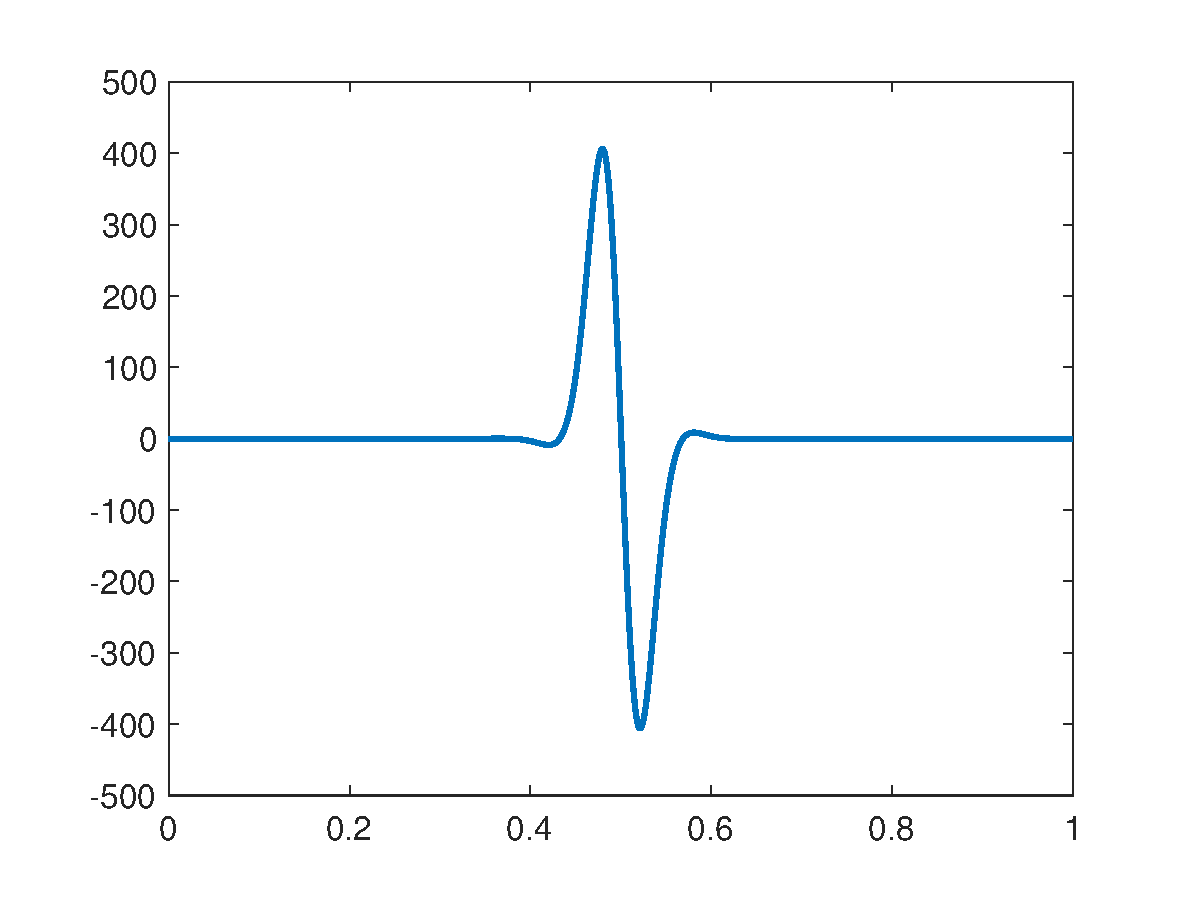
\includegraphics[width=6cm]{images/kdv5numerics/single10derivative} &
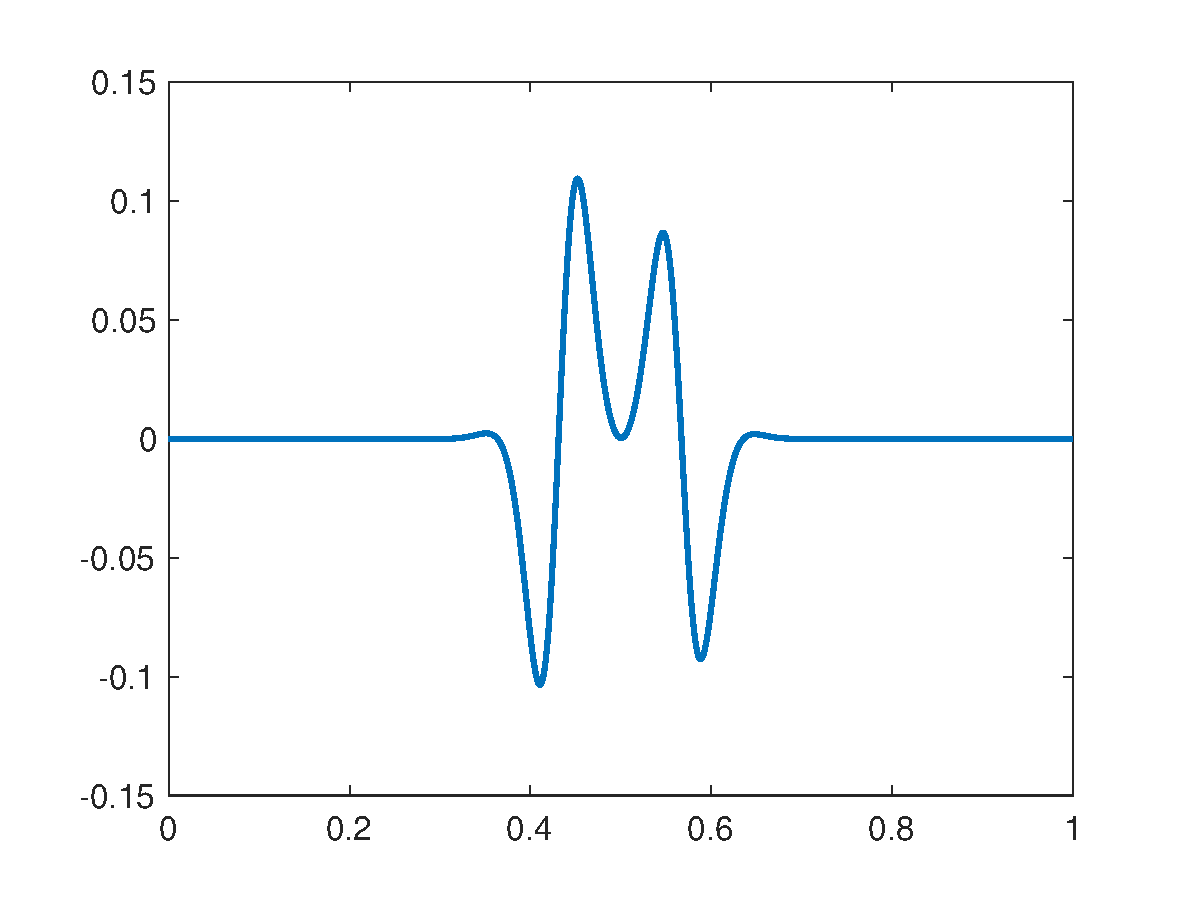
\includegraphics[width=6cm]{images/kdv5numerics/double1inteigfunction} \\
\end{tabular}
\caption[Interaction eigenfunctions for double pulses in KdV5]{Plot of derivative of primary pulse (left) and interaction eigenfunction for first double pulse (right). Fourier spectral methods with $N = 1024$ grid points, $c = 10$, $L = 25$.}
\label{fig:KdV5inteigplot}
\end{center}
\end{figure}

Before we continue, we note that all the eigenvalue computations thus far have relied on Fourier differentiation matrices; in doing this, we have posed the problem with periodic boundary conditions. Since we have chosen the scaling parameter $L$ sufficiently large so that the tails of the pulses have sufficient room to decay, this should approximate the situation on the entire real line. We can repeat the above using separated boundary conditions. A convenient choice for this is Chebyshev polynomial spectral methods with Dirichlet and Neumann boundary conditions at the endpoints. When we do this, we obtain the same interaction eigenvalues that we did with Fourier spectral methods. The main difference is that the matrix eigenvalues representing the essential spectrum have shifted to the right half plane. This is shown for the second double pulse in \cref{fig:KdV5speccheb}. As the domain scaling parameter $L \rightarrow \infty$, these eigenvalues should approach the absolute spectrum.
\begin{figure}
\begin{center}
\begin{tabular}{cc}
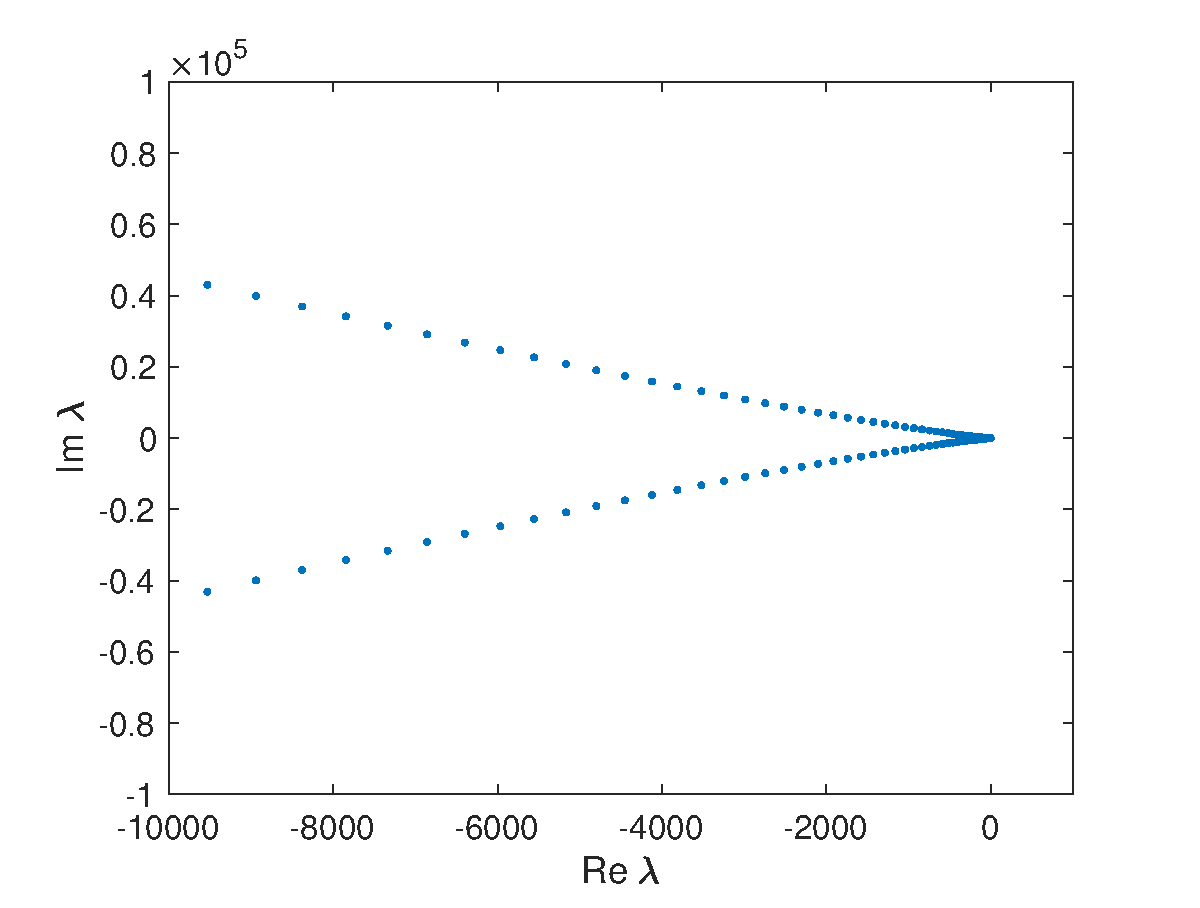
\includegraphics[width=6cm]{images/kdv5numerics/double2speccheb} &
\includegraphics[width=6cm]{images/kdv5numerics/double2specchebzoom.eps} \\
\end{tabular}
\caption[Spectrum of double pulses in KdV5 (Chebyshev spectral methods)]{Spectrum of $\partial_x \calE''(q_2)$ for second double pulse (left) with zoom in around origin showing interaction eigenvalues (right). Chebyshev spectral methods, $N = 512$ grid points, $c = 10$, $L = 25$.}
\label{fig:KdV5speccheb}
\end{center}
\end{figure}
Since there is no essential spectrum in the way, it may be easier to find the interaction eigenvalues using Chebyshev polynomial spectral methods.

\subsection{Time stepping}

In this section, we perform time-stepping of the PDE \eqref{KdV5c} starting with initial conditions which are near to the double pulse equilibrium solutions we constructed earlier. For spatial discretization we use Chebyshev spectral methods. This avoids the small-amplitude oscillatory modes which come from the purely imaginary essential spectrum in the case of periodic boundary conditions. For time-stepping, we use a Crank-Nicolson/Adams-Bashforth 2 (CNAB) IMEX scheme. To obtain an initial condition near a double pulse, we ``pull apart'' the two pulses by inserting a small flat segment at the origin (which is exactly half way between the two pulses). We do this for many initial conditions near the first four double pulses. For each point in time, we compute the peak distance and its derivative, which we will call the pulse relative velocity. Trajectories of this two-dimensional system are plotted in the left panel of \cref{fig:KdV5timestep}
\begin{figure}
\begin{center}
\begin{tabular}{cc}
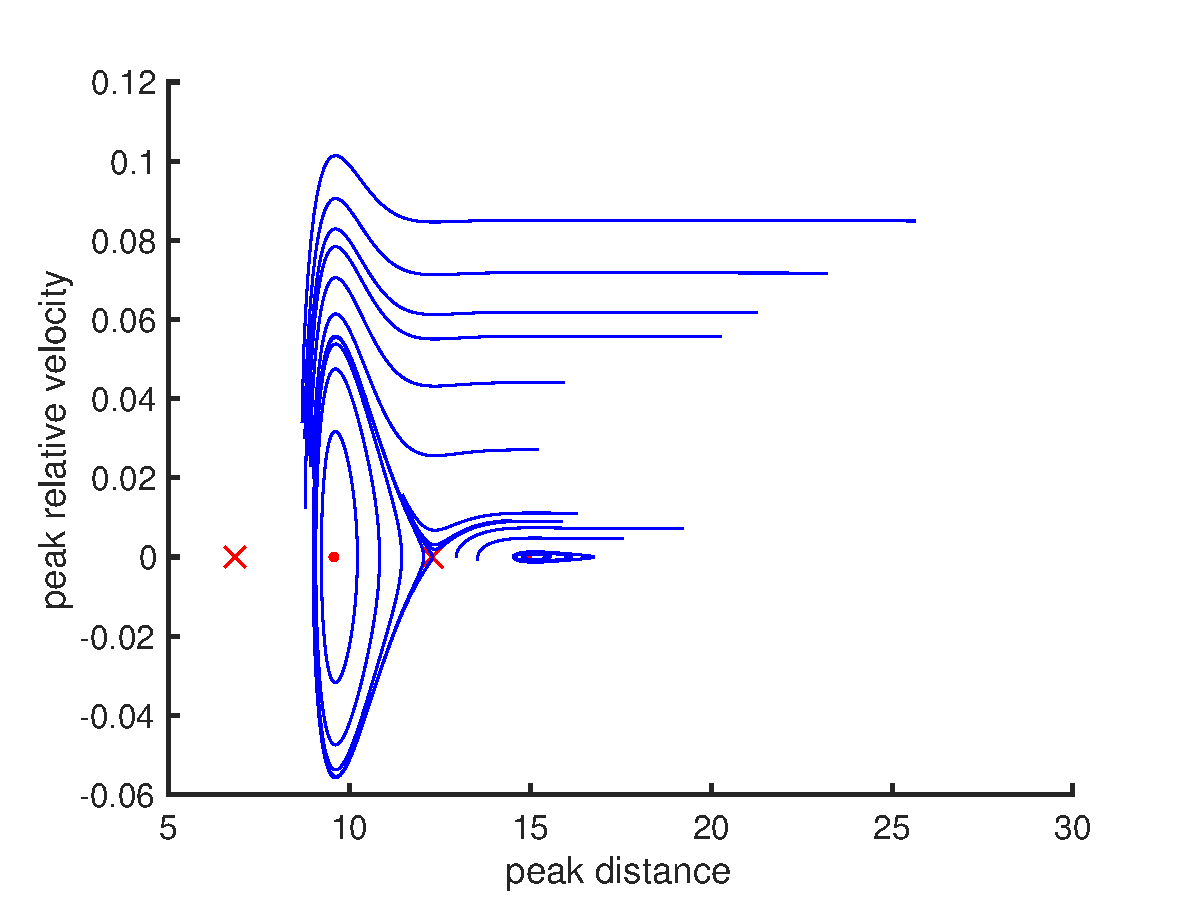
\includegraphics[width=8cm]{images/kdv5numerics/phaseportrait} &
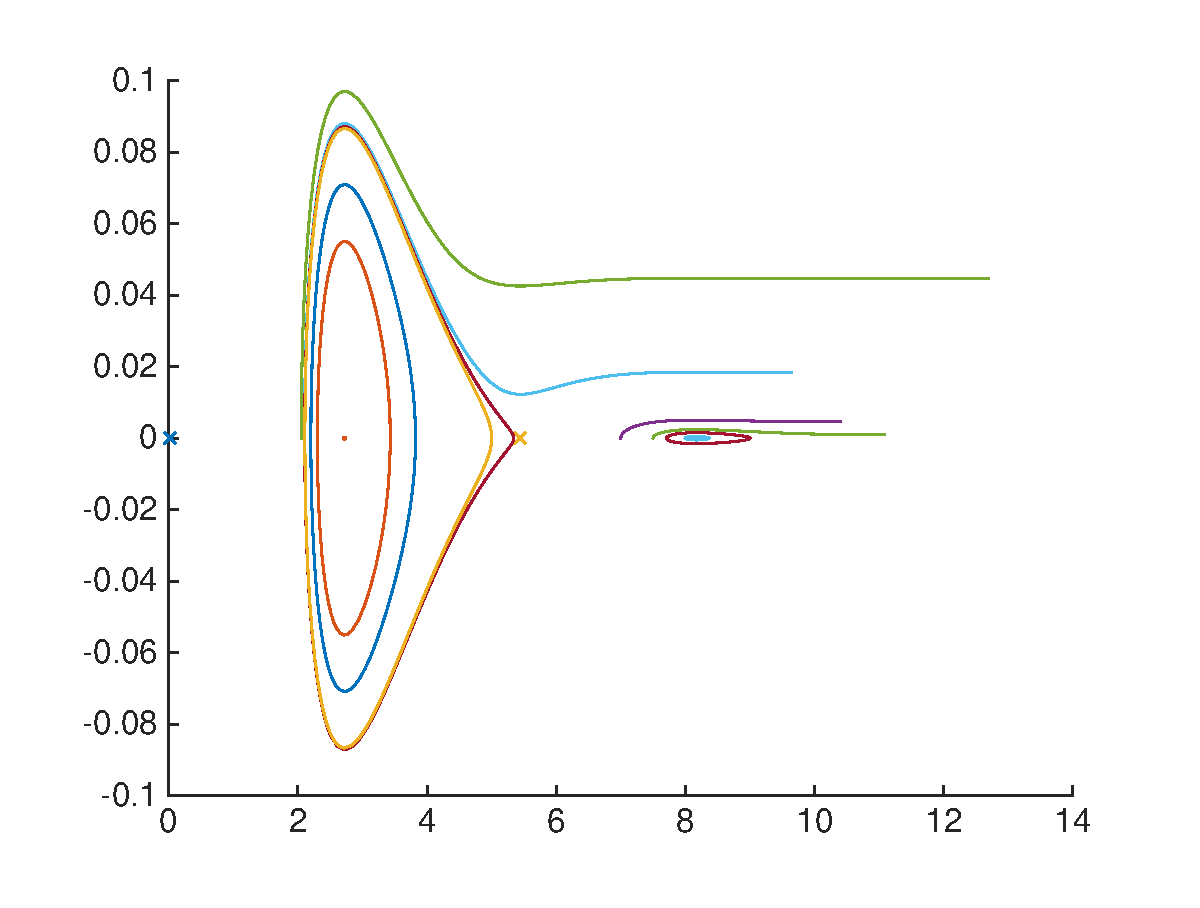
\includegraphics[width=8cm]{images/kdv5numerics/simplephaseportrait} \\
\end{tabular}
\caption[Phase portraits for timestepping of double pulses in KdV5]{Phase portrait for peak relative velocity vs. peak distance for timestepping of \cref{KdV5c} with initial conditions near the first four double pulses (left panel). Phase portrait of \cref{harmonicvary} (right panel). For left panel, we used Chebyshev spectral methods, $N = 512$ grid points, $c = 10$, $L = 25$. Right panel is generated using Matlab's \texttt{ode45} function.
}
\label{fig:KdV5timestep}
\end{center}
\end{figure}
This phase portrait consists of alternating saddles and centers and resembles a harmonic oscillator with spatially varying restoring force. In fact, we can construct a such an oscillator with the following planar system
\begin{equation}\label{harmonicvary}
\begin{aligned}
\dot{x} &= y \\
\dot{y} &= C e^{-\alpha_0 x} \sin \beta_0 x
\end{aligned}
\end{equation}
where we recall that $\pm \alpha_0 \pm \beta_0 i$ are the nonzero eigenvalues of the rest state. The phase portrait for this system is plotted in the right panel of \cref{fig:KdV5timestep}. We note the similarity between the two phase portraits.

\subsection{Periodic multi-pulses}

We will now consider solutions on a periodic domain. A periodic multi-pulse is a multi-pulse solution to \cref{KdV5eq4} with periodic boundary conditions. In the previous section, we used Fourier spectral methods with periodic boundary conditions, so technically all of those solutions are periodic multi-pulses. However, we chose the period sufficiently large to approximate the situation on the real line but not too large to cause problems. Here we will look periodic double pulses in the two extreme cases: small period, where the interaction between two two pulses pulses is significant on both sides, and large period, where there is a collision between eigenvalues on the imaginary axis.

Before we continue, we note that for the operator $\partial_x \calE''(q_n)$ on the real line, the essential spectrum consists of the entire imaginary axis. When we shift to a periodic domain, the essential spectrum becomes a collection of discrete, purely imaginary eigenvalues. These only depend on the size of the periodic domain. For periodic domain $[-L, L]$, these eigenvalues are located at approximately
\begin{equation}\label{Kdv5peress}
\lambda \approx \left\{ c \frac{k \pi i}{L} : k \in \Z \right\} ,
\end{equation}
where $c$ is the wavespeed.

First, we look at the small period case. Using AUTO, we start with the double pulses constructed in the previous section, and decrease the domain length parameter $L$. Transforming back from the interval $[0, 1]$ to $[-L, L]$, we plot the pulse distances $2 X_0$ vs $2 X_1$ in \cref{fig:periodicpitchfork}.
\begin{figure}
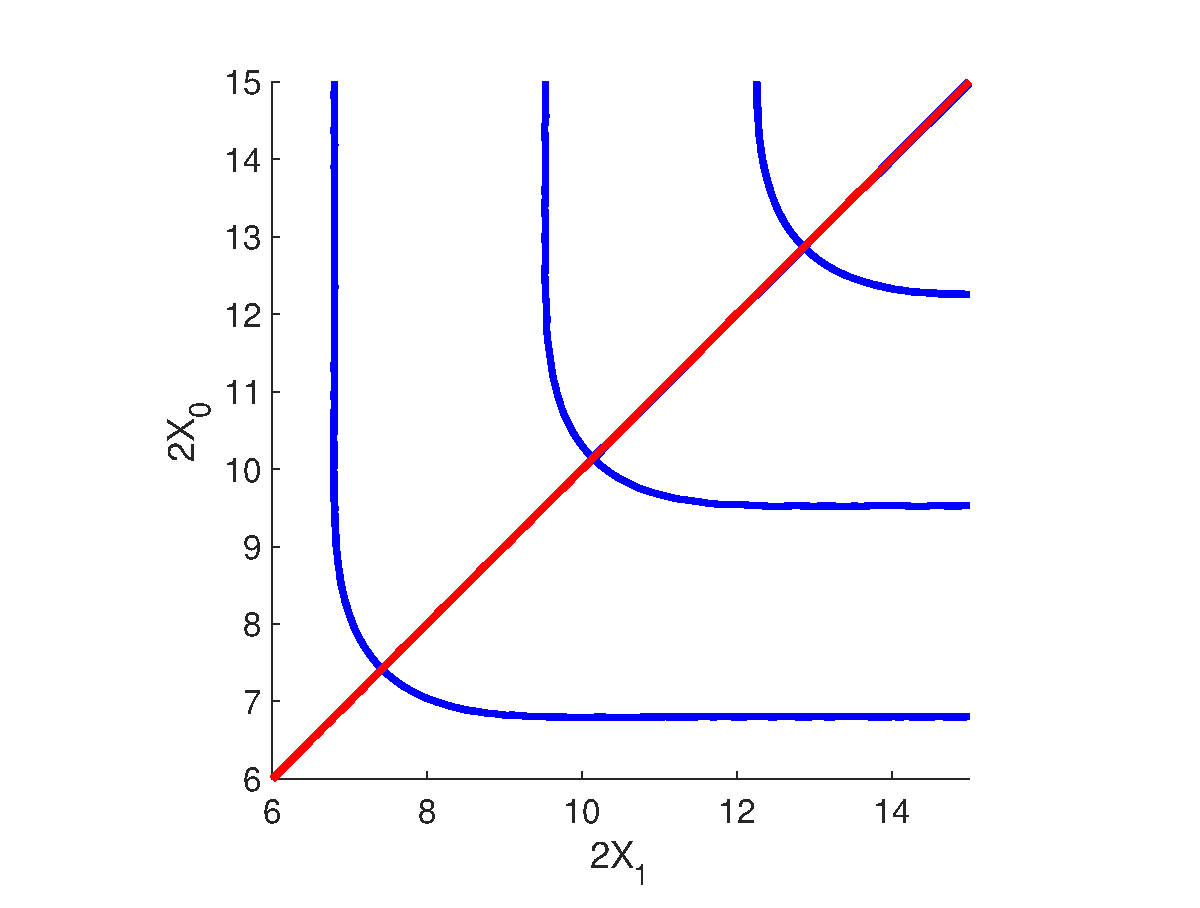
\includegraphics[width=10cm]{images/kdv5numerics/periodicpitchfork.eps}
\caption[Pulse distances of periodic multi-pulses in KdV5]{Pulse distances $2 X_0$ vs $2 X_1$ for periodic double pulse solutions to \cref{KdV5eq4}. Solutions with unequal pulse distances corresponding to the first three double pulses are shown in blue. Solutions with equal pulse distances are shown in red.}
\label{fig:periodicpitchfork}
\end{figure}
From this figure, we see that solutions with unequal pulse distances bifurcate from solutions with equal pulse distances in a series of pitchfork bifurcations. Next, we compute the interaction eigenvalues for the periodic 2-pulses with equal pulse distances. The result is shown in \cref{fig:periodicequaleigbif}.
\begin{figure}
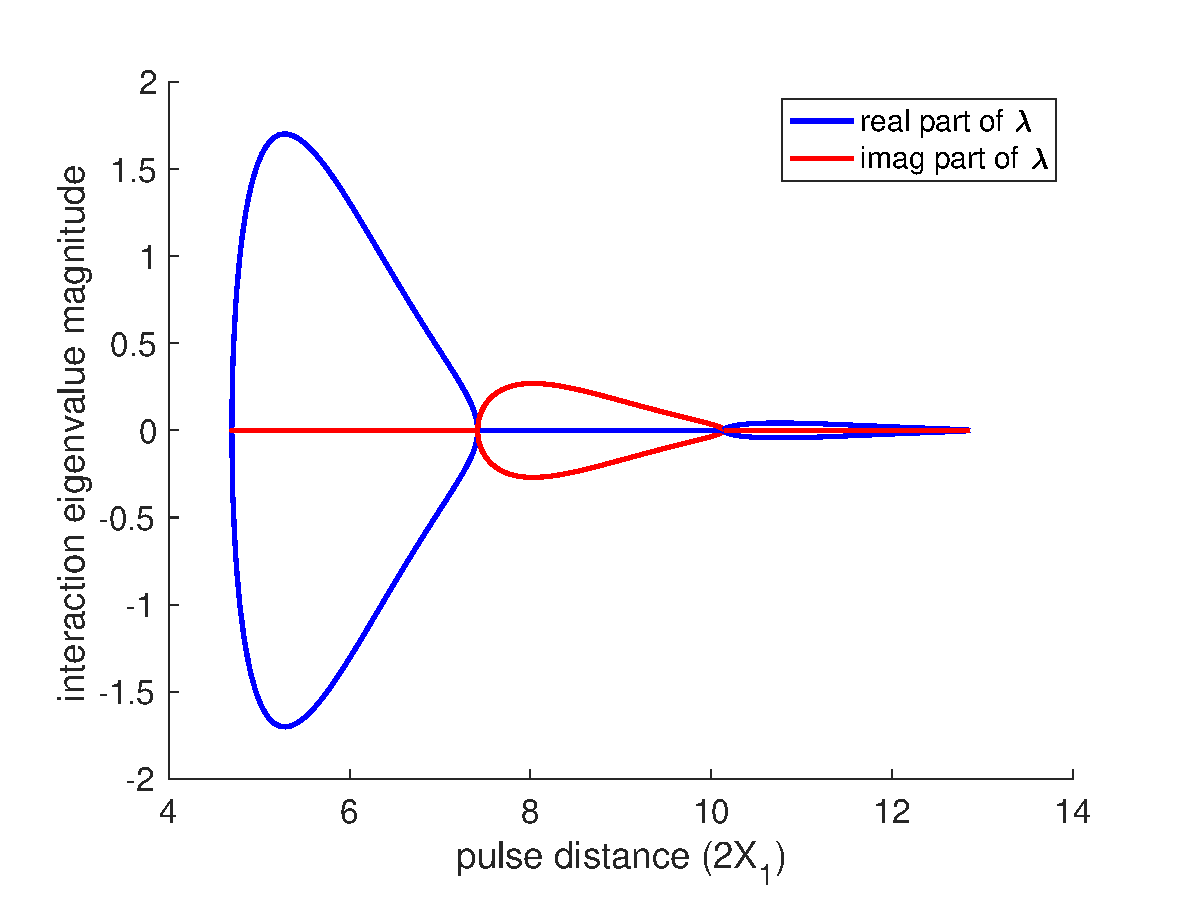
\includegraphics[width=10cm]{images/kdv5numerics/periodicequaleigbif.eps}
\caption[Eigenvalue bifurcations for symmetric periodic double pulses in KdV5]{Real (blue line) and imaginary (red line) parts of interaction eigenvalues versus pulse distance ($2 X_1$) for periodic 2-pulses with equal pulse distances.}
\label{fig:periodicequaleigbif}
\end{figure}
At each of the pitchfork bifurcation points in \cref{fig:periodicpitchfork}, an eigenvalue bifurcation occurs, where a pair of interaction eigenvalues collides at 0 and switches from real to purely imaginary (or vice versa). The full interaction eigenvalue pattern corresponding to \cref{fig:periodicpitchfork} is given in \cref{fig:2periodiceigpattern}.

\begin{figure}
\includegraphics[width=10cm]{images/kdv5numerics/2periodiceigpattern.eps}
\caption[Interaction eigenvalue pattern for periodic double pulses in KdV5]{Interaction eigenvalue pattern for periodic 2-pulses. Blue lines represent periodic 2-pulses with a pair of real interaction eigenvalues. Red lines represent periodic 2-pulses with a pair of purely imaginary interaction eigenvalues. Hamiltonian-Hopf bifurcations take place in the interaction eigenvalues at the black dots.}
\label{fig:2periodiceigpattern}
\end{figure}

Finally, we look at what happens when we increase the period $L$. For a neutrally stable double pulse, we have a pair of interaction eigenvalues on the imaginary axis whose location is approximately constant for sufficiently large $L$. On the other hand, the essential spectrum eigenvalues \cref{Kdv5peress} move towards the origin as $L$ is increased. It is straightforward to determine the Krein signatures of the eigenvalues numerically; the interaction eigenvalues have negative Krein signature and the essential spectrum eigenvalues have positive Krein signature. At some value of $L$, these eigenvalues will collide. When this happens, since the two eigenvalues have opposite Krein signatures, the two eigenvalues will generically move off of the imaginary axis and create an instability \cite[Chapter 7.1]{Kapitula2013}. By Hamiltonian symmetry, we expect there to be a pair of eigenvalues which has nonzero real part and is symmetric across the imaginary axis.

To see what happens, we increase the periodic length parameter $L$ using AUTO. This is shown in \cref{fig:kreinbubble1}.
\begin{figure}
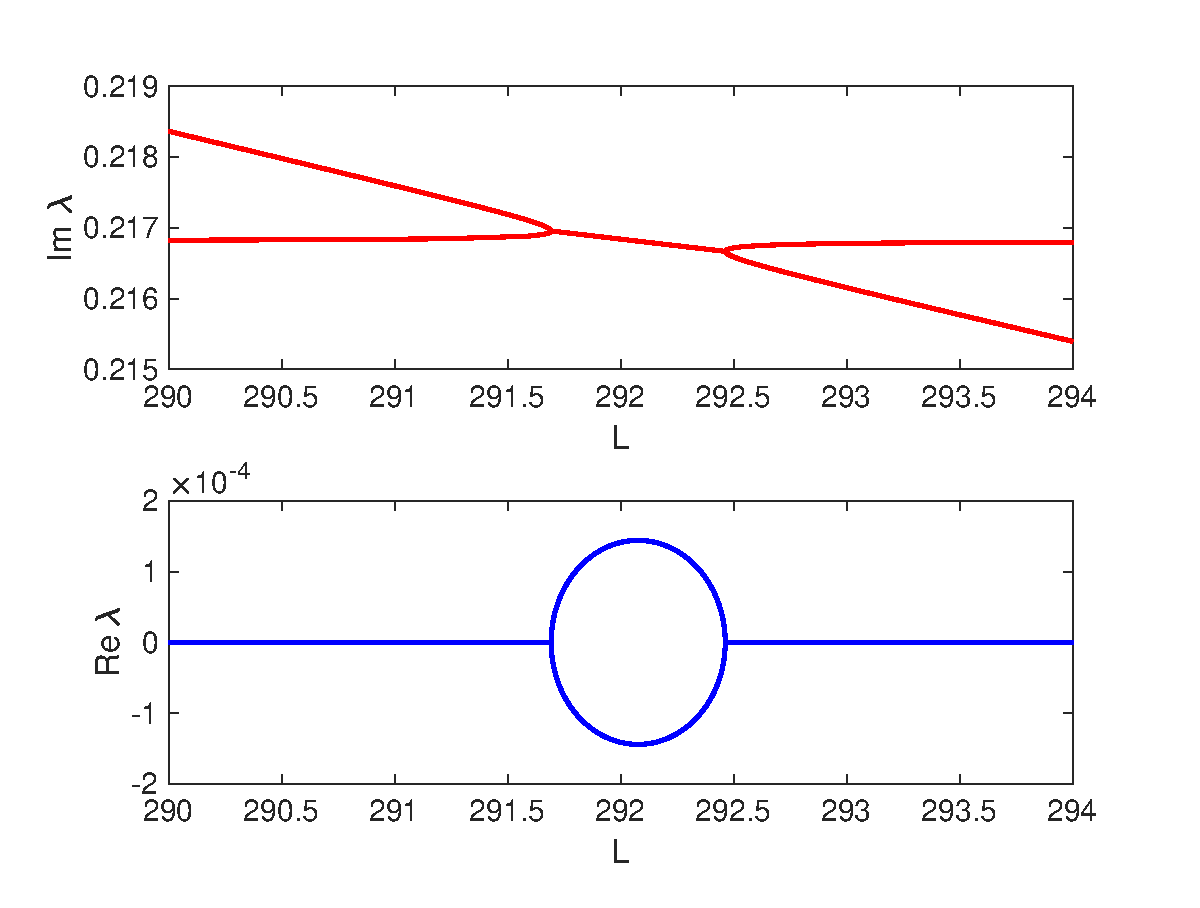
\includegraphics[width=10cm]{images/kdv5numerics/kreinbubble1}
\caption[Eigenvalue collisions for periodic double pulses in KdV5]{Collision of first essential spectrum eigenvalue with purely imaginary interaction eigenvalue as $L$ is increased. Imaginary part of eigenvalues on top, real part of eigenvalues on bottom. Parameter continuation with AUTO in periodic domain length $L$, $c = 20$.}
\label{fig:kreinbubble1}
\end{figure}
As $L$ is increased, the two eigenvalues undergo a Krein collision and move off of the imaginary axis. The real part of the eigenvalue post-collision is very small compared to the imaginary part, approximately order $10^{-4}$. As $L$ is further increased, the eigenvalues come back together on the imaginary axis in a reverse Krein collision. Increasing $L$ further, the essential spectrum eigenvalue continues to move on the imaginary axis towards the origin, and the interaction eigenvalue is unchanged. We will call this instability bubble a Krein bubble. \cref{fig:kreinbubble1zoom} shows the eigenvalues of the Krein bubble in the complex plane. To leading order, the bubble is a circle.
\begin{figure}
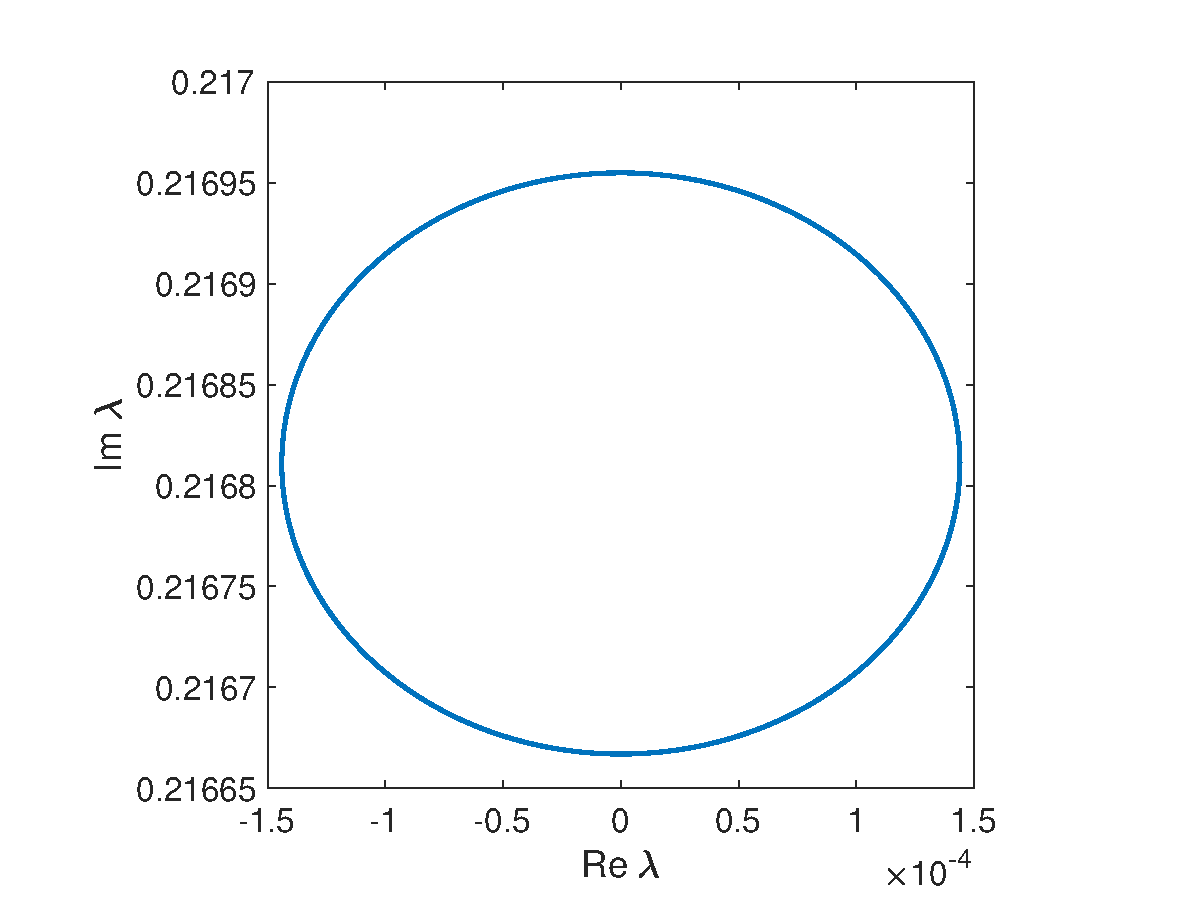
\includegraphics[width=10cm]{images/kdv5numerics/kreinbubble1zoom}
\caption[First Krein bubble for KdV5]{Plot of imaginary vs real part of eigenvalues inside Krein bubble occurring upon collision of first essential spectrum eigenvalue with interaction eigenvalue. $c = 20$.}
\label{fig:kreinbubble1zoom}
\end{figure}
We can continue the parameter continuation with AUTO, and we find a Krein bubble with every subsequent collision of an essential spectrum eigenvalue with the interaction eigenvalue. \cref{fig:kreinbubbleradius} plots the log of the Krein bubble radius versus the log of $L$ for the first 10 Krein bubbles.
\begin{figure}
\includegraphics[width=10cm]{images/kdv5numerics/kreinbubbleradius}
\caption[Krein bubble radius for KdV5]{Plot of log of Krein bubble radius vs. log $L$ for the first 10 Krein bubbles together with least squares linear regression line. $c = 20$.}
\label{fig:kreinbubbleradius}
\end{figure}
The slope of the least squares linear regression line is $-0.5$ (with a relative error of less than $0.005$), which suggests that the radius of the Krein bubble scales as $L^{-1/2}$.

\iffulldocument\else
	\bibliographystyle{amsalpha}
	\bibliography{thesis2.bib}
\fi

\end{document}